% Options for packages loaded elsewhere
\PassOptionsToPackage{unicode}{hyperref}
\PassOptionsToPackage{hyphens}{url}
%
\documentclass[
]{article}
\usepackage{lmodern}
\usepackage{amssymb,amsmath}
\usepackage{ifxetex,ifluatex}
\ifnum 0\ifxetex 1\fi\ifluatex 1\fi=0 % if pdftex
  \usepackage[T1]{fontenc}
  \usepackage[utf8]{inputenc}
  \usepackage{textcomp} % provide euro and other symbols
\else % if luatex or xetex
  \usepackage{unicode-math}
  \defaultfontfeatures{Scale=MatchLowercase}
  \defaultfontfeatures[\rmfamily]{Ligatures=TeX,Scale=1}
\fi
% Use upquote if available, for straight quotes in verbatim environments
\IfFileExists{upquote.sty}{\usepackage{upquote}}{}
\IfFileExists{microtype.sty}{% use microtype if available
  \usepackage[]{microtype}
  \UseMicrotypeSet[protrusion]{basicmath} % disable protrusion for tt fonts
}{}
\makeatletter
\@ifundefined{KOMAClassName}{% if non-KOMA class
  \IfFileExists{parskip.sty}{%
    \usepackage{parskip}
  }{% else
    \setlength{\parindent}{0pt}
    \setlength{\parskip}{6pt plus 2pt minus 1pt}}
}{% if KOMA class
  \KOMAoptions{parskip=half}}
\makeatother
\usepackage{xcolor}
\IfFileExists{xurl.sty}{\usepackage{xurl}}{} % add URL line breaks if available
\IfFileExists{bookmark.sty}{\usepackage{bookmark}}{\usepackage{hyperref}}
\hypersetup{
  hidelinks,
  pdfcreator={LaTeX via pandoc}}
\urlstyle{same} % disable monospaced font for URLs
\usepackage{color}
\usepackage{fancyvrb}
\newcommand{\VerbBar}{|}
\newcommand{\VERB}{\Verb[commandchars=\\\{\}]}
\DefineVerbatimEnvironment{Highlighting}{Verbatim}{commandchars=\\\{\}}
% Add ',fontsize=\small' for more characters per line
\newenvironment{Shaded}{}{}
\newcommand{\AlertTok}[1]{\textcolor[rgb]{1.00,0.00,0.00}{\textbf{#1}}}
\newcommand{\AnnotationTok}[1]{\textcolor[rgb]{0.38,0.63,0.69}{\textbf{\textit{#1}}}}
\newcommand{\AttributeTok}[1]{\textcolor[rgb]{0.49,0.56,0.16}{#1}}
\newcommand{\BaseNTok}[1]{\textcolor[rgb]{0.25,0.63,0.44}{#1}}
\newcommand{\BuiltInTok}[1]{#1}
\newcommand{\CharTok}[1]{\textcolor[rgb]{0.25,0.44,0.63}{#1}}
\newcommand{\CommentTok}[1]{\textcolor[rgb]{0.38,0.63,0.69}{\textit{#1}}}
\newcommand{\CommentVarTok}[1]{\textcolor[rgb]{0.38,0.63,0.69}{\textbf{\textit{#1}}}}
\newcommand{\ConstantTok}[1]{\textcolor[rgb]{0.53,0.00,0.00}{#1}}
\newcommand{\ControlFlowTok}[1]{\textcolor[rgb]{0.00,0.44,0.13}{\textbf{#1}}}
\newcommand{\DataTypeTok}[1]{\textcolor[rgb]{0.56,0.13,0.00}{#1}}
\newcommand{\DecValTok}[1]{\textcolor[rgb]{0.25,0.63,0.44}{#1}}
\newcommand{\DocumentationTok}[1]{\textcolor[rgb]{0.73,0.13,0.13}{\textit{#1}}}
\newcommand{\ErrorTok}[1]{\textcolor[rgb]{1.00,0.00,0.00}{\textbf{#1}}}
\newcommand{\ExtensionTok}[1]{#1}
\newcommand{\FloatTok}[1]{\textcolor[rgb]{0.25,0.63,0.44}{#1}}
\newcommand{\FunctionTok}[1]{\textcolor[rgb]{0.02,0.16,0.49}{#1}}
\newcommand{\ImportTok}[1]{#1}
\newcommand{\InformationTok}[1]{\textcolor[rgb]{0.38,0.63,0.69}{\textbf{\textit{#1}}}}
\newcommand{\KeywordTok}[1]{\textcolor[rgb]{0.00,0.44,0.13}{\textbf{#1}}}
\newcommand{\NormalTok}[1]{#1}
\newcommand{\OperatorTok}[1]{\textcolor[rgb]{0.40,0.40,0.40}{#1}}
\newcommand{\OtherTok}[1]{\textcolor[rgb]{0.00,0.44,0.13}{#1}}
\newcommand{\PreprocessorTok}[1]{\textcolor[rgb]{0.74,0.48,0.00}{#1}}
\newcommand{\RegionMarkerTok}[1]{#1}
\newcommand{\SpecialCharTok}[1]{\textcolor[rgb]{0.25,0.44,0.63}{#1}}
\newcommand{\SpecialStringTok}[1]{\textcolor[rgb]{0.73,0.40,0.53}{#1}}
\newcommand{\StringTok}[1]{\textcolor[rgb]{0.25,0.44,0.63}{#1}}
\newcommand{\VariableTok}[1]{\textcolor[rgb]{0.10,0.09,0.49}{#1}}
\newcommand{\VerbatimStringTok}[1]{\textcolor[rgb]{0.25,0.44,0.63}{#1}}
\newcommand{\WarningTok}[1]{\textcolor[rgb]{0.38,0.63,0.69}{\textbf{\textit{#1}}}}
\usepackage{graphicx,grffile}
\makeatletter
\def\maxwidth{\ifdim\Gin@nat@width>\linewidth\linewidth\else\Gin@nat@width\fi}
\def\maxheight{\ifdim\Gin@nat@height>\textheight\textheight\else\Gin@nat@height\fi}
\makeatother
% Scale images if necessary, so that they will not overflow the page
% margins by default, and it is still possible to overwrite the defaults
% using explicit options in \includegraphics[width, height, ...]{}
\setkeys{Gin}{width=\maxwidth,height=\maxheight,keepaspectratio}
% Set default figure placement to htbp
\makeatletter
\def\fps@figure{htbp}
\makeatother
\setlength{\emergencystretch}{3em} % prevent overfull lines
\providecommand{\tightlist}{%
  \setlength{\itemsep}{0pt}\setlength{\parskip}{0pt}}
\setcounter{secnumdepth}{-\maxdimen} % remove section numbering

\date{}

\begin{document}

\hypertarget{header-n0}{%
\section{SE-344}\label{header-n0}}

\hypertarget{header-n2}{%
\subsection{Assignment \#2 Report}\label{header-n2}}

\begin{itemize}
\item
  姓名:于喜千
\item
  学号:\texttt{517030910168}
\item
  任务:Assignment \#2
\end{itemize}

\hypertarget{header-n10}{%
\subsubsection{过程描述}\label{header-n10}}

\hypertarget{header-n11}{%
\paragraph{第一部分:搭建 OpenGL 编程环境}\label{header-n11}}

\hypertarget{header-n12}{%
\subparagraph{环境设定}\label{header-n12}}

\begin{itemize}
\item
  Windows 10 x64 LTSC 1809 (\texttt{17763.737})
\item
  Visual Studio 2019 Community (\texttt{16.2.4})
\item
  FreeGLUT
\end{itemize}

此处,比照 Assignment \#1 中的环境设定办理。

\hypertarget{header-n21}{%
\paragraph{第二部分:数据处理}\label{header-n21}}

由于本次 Assignment 中的三角形数据来自 \texttt{overlapping.tri} 和
\texttt{intersecting.tri},因此我们首先需要实现三角形数据的读取。

\hypertarget{header-n23}{%
\subparagraph{标准库使用}\label{header-n23}}

这里,主要利用了 C++ 中的 \texttt{\textless{}fstream\textgreater{}} 和
\texttt{\textless{}iostream\textgreater{}} 标准库来实现文件数据的读取。

\hypertarget{header-n25}{%
\subparagraph{数据格式}\label{header-n25}}

在作业提供的 \texttt{.tri} 文件中,包含由不定数量的空格符及
\texttt{\textquotesingle{}\textbackslash{}n\textquotesingle{}}
分隔的数字;这些数字依次代表了三角形每个顶点的 x、y、z
坐标位置(有符号整数)及 R、G、B 颜色分量(0 ~ 1 之间的浮点数)。

文件以 \texttt{\textquotesingle{}\textbackslash{}n\textquotesingle{}} +
EOF 结束。

\hypertarget{header-n28}{%
\subparagraph{程序结构}\label{header-n28}}

相关文件包括 \texttt{Triangle.hpp}、\texttt{Reader.h}、和
\texttt{Reader.cpp}。

在 \texttt{Triangle.hpp} 中,定义着 \texttt{TrianglePoint} 和
\texttt{Triangle}
两个类;他们用于结构化地描述三角形的顶点位置及顶点颜色。同时,提供了默认的无参构造函数及完整构造函数,方便各种形式的调用;同时在构造时还对
R、G、B 颜色分量进行了范围检测和归一化纠错,减少错误调用的可能性。

在 \texttt{Reader.cpp} + \texttt{Reader.h} 两个文件中,定义了一个名为
\texttt{readTriangle}
的参数;它可以通过提供文件名作为参数来读取所有满足上述条件的
\texttt{.tri} 文件,并将其放置在
\texttt{vector\textless{}Triangle\textgreater{}}
中并返回。这就意味着我们可以在随后的 Phases
中复用这个函数,减少重复工作,提高程序效能。

\hypertarget{header-n32}{%
\subparagraph{执行结果}\label{header-n32}}

通过断点调试方法,发现程序可以成功处理 \texttt{overlapping.tri} 和
\texttt{intersecting.tri} 两个 \texttt{.tri} 文件,并能正确生成
\texttt{Triangle} 对象。

\hypertarget{header-n34}{%
\paragraph{第三部分:三角形绘制}\label{header-n34}}

\hypertarget{header-n35}{%
\subparagraph{程序结构}\label{header-n35}}

这一部分的代码更改主要在 \texttt{main.cpp}
的渲染部分。另外,扫描线算法的实现位于 \texttt{DepthChecker.hpp} 中。

首先,我们引入 \texttt{Triangle.hpp} 及 \texttt{Reader.h}
头文件来读入所需的文件。

\hypertarget{header-n38}{%
\subparagraph{读取数据}\label{header-n38}}

\begin{Shaded}
\begin{Highlighting}[]
\KeywordTok{auto}\NormalTok{ triangles = readTriangle(}\StringTok{"./overlapping.tri"}\NormalTok{);}
\CommentTok{/* 'triangles' type: std::vector<Triangles> */}
\end{Highlighting}
\end{Shaded}

由于除错调试时的 \texttt{.tri}
文件路径和实际运行时的路径有出入,因此为了保证程序灵活性,采用运行时指定文件路径的做法,如此:

\begin{Shaded}
\begin{Highlighting}[]
\BuiltInTok{std::}\NormalTok{cin >> path;}
\KeywordTok{auto}\NormalTok{ triangles = readTriangle(path);}
\end{Highlighting}
\end{Shaded}

\hypertarget{header-n42}{%
\subparagraph{绘制三角形}\label{header-n42}}

为了减少代码绘制时产生的问题,这里复用了上一次的视角旋转代码来实现视角的改变。

同样,绘制图形的代码在 \texttt{onRender()} 函数中实现。

启用深度检测

在 \texttt{main} 函数中,我们使用下列方法来启用深度检测:

\begin{Shaded}
\begin{Highlighting}[]
\CommentTok{// 设置深度缓存}
\NormalTok{glClearDepth(}\FloatTok{1.0}\NormalTok{);}

\CommentTok{// 启用深度测试}
\NormalTok{glEnable(GL_DEPTH_TEST);}

\CommentTok{// 所作深度测试的类型}
\NormalTok{glDepthFunc(GL_LEQUAL);}

\CommentTok{// 启用平滑}
\NormalTok{glShadeModel(GL_SMOOTH);}
\end{Highlighting}
\end{Shaded}

关键方法为 \texttt{glEnable(GL\_DEPTH\_TEST)},该函数启用了 GLUT
提供的深度测试。

留意到我们需要使用重心差值渐变来绘制三角形,因此我们调用
\texttt{glShadeModel(GL\_SMOOTH)} 函数。

而 \texttt{glDepthFunc(...)}
函数可以指定进行深度测试的类型。可以使用的参数包括:

\begin{itemize}
\item
  \texttt{GL\_NEVER}, 总是不通过(输入的深度值不取代参考值)
\item
  \texttt{GL\_LESS}, 如果输入的深度值小于参考值,则通过
\item
  \texttt{GL\_EQUAL}, 如果输入的深度值等于参考值,则通过
\item
  \texttt{GL\_LEQUAL}, 如果输入的深度值小于或等于参考值,则通过
\item
  \texttt{GL\_GREATER}, 如果输入的深度值大于参考值,则通过
\item
  \texttt{GL\_NOTEQUAL}, 如果输入的深度值不等于参考值,则通过
\item
  \texttt{GL\_GEQUAL}, 如果输入的深度值大于或等于参考值,则通过
\item
  \texttt{GL\_ALWAYS}, 总是通过(输入的深度值取代参考值)
\end{itemize}

(Refs: glDepthFunc - OpenGL 4 Reference Pages)

清除缓存

由于开启了深度检测,因此我们在每次开始渲染时,不仅要清除像素缓存
Bit(\texttt{GL\_COLOR\_BUFFER\_BIT}),同时还要清除深度缓存
Bit(\texttt{GL\_DEPTH\_BUFFER\_BIT})。

\begin{Shaded}
\begin{Highlighting}[]
\NormalTok{glClear(GL_COLOR_BUFFER_BIT | GL_DEPTH_BUFFER_BIT);}
\end{Highlighting}
\end{Shaded}

绘制三角形

因为我们已经得到了 \texttt{Triangle} 数组,因此只需要使用
\texttt{glBegin(GL\_TRIANGLES)} 来绘制就好了。

在 \texttt{glBegin} 和 \texttt{glEnd} 之间,连续调用 \texttt{glColor3d}
和 \texttt{glVertex3d} 来绘制不同颜色的顶点。

绘制参考线

\begin{Shaded}
\begin{Highlighting}[]
\NormalTok{glColor3d(}\FloatTok{0.6}\NormalTok{, }\FloatTok{0.6}\NormalTok{, }\FloatTok{0.7}\NormalTok{);}
\ControlFlowTok{for}\NormalTok{ (}\DataTypeTok{float}\NormalTok{ i = -}\DecValTok{50}\NormalTok{; i <= }\DecValTok{50}\NormalTok{; i += }\FloatTok{0.2}\BuiltInTok{f}\NormalTok{)}
\NormalTok{\{}
	\CommentTok{/** 绘制线 */}
\NormalTok{	glBegin(GL_LINES);}

	\CommentTok{/** x 轴方向 */}
\NormalTok{	glVertex3f(-}\DecValTok{50}\NormalTok{, }\DecValTok{0}\NormalTok{, i);}
\NormalTok{	glVertex3f(}\DecValTok{50}\NormalTok{, }\DecValTok{0}\NormalTok{, i);}

	\CommentTok{/** z 轴方向 */}
\NormalTok{	glVertex3f(i, }\DecValTok{0}\NormalTok{, -}\DecValTok{50}\NormalTok{);}
\NormalTok{	glVertex3f(i, }\DecValTok{0}\NormalTok{, }\DecValTok{50}\NormalTok{);}

\NormalTok{	glEnd();}
\NormalTok{\}}
\end{Highlighting}
\end{Shaded}

为了保证空间视觉观看体验,因此我们在 xOz
平面上绘制一系列的灰色网格来帮助我们观察。

\hypertarget{header-n78}{%
\subparagraph{观察结果}\label{header-n78}}

根据程序读取 \texttt{overlapping.tri} 和 \texttt{intersecting.tri}
的结果来看,可以看出 OpenGL 提供的深度检测算法表现优异,运行高效。

\begin{figure}
\centering
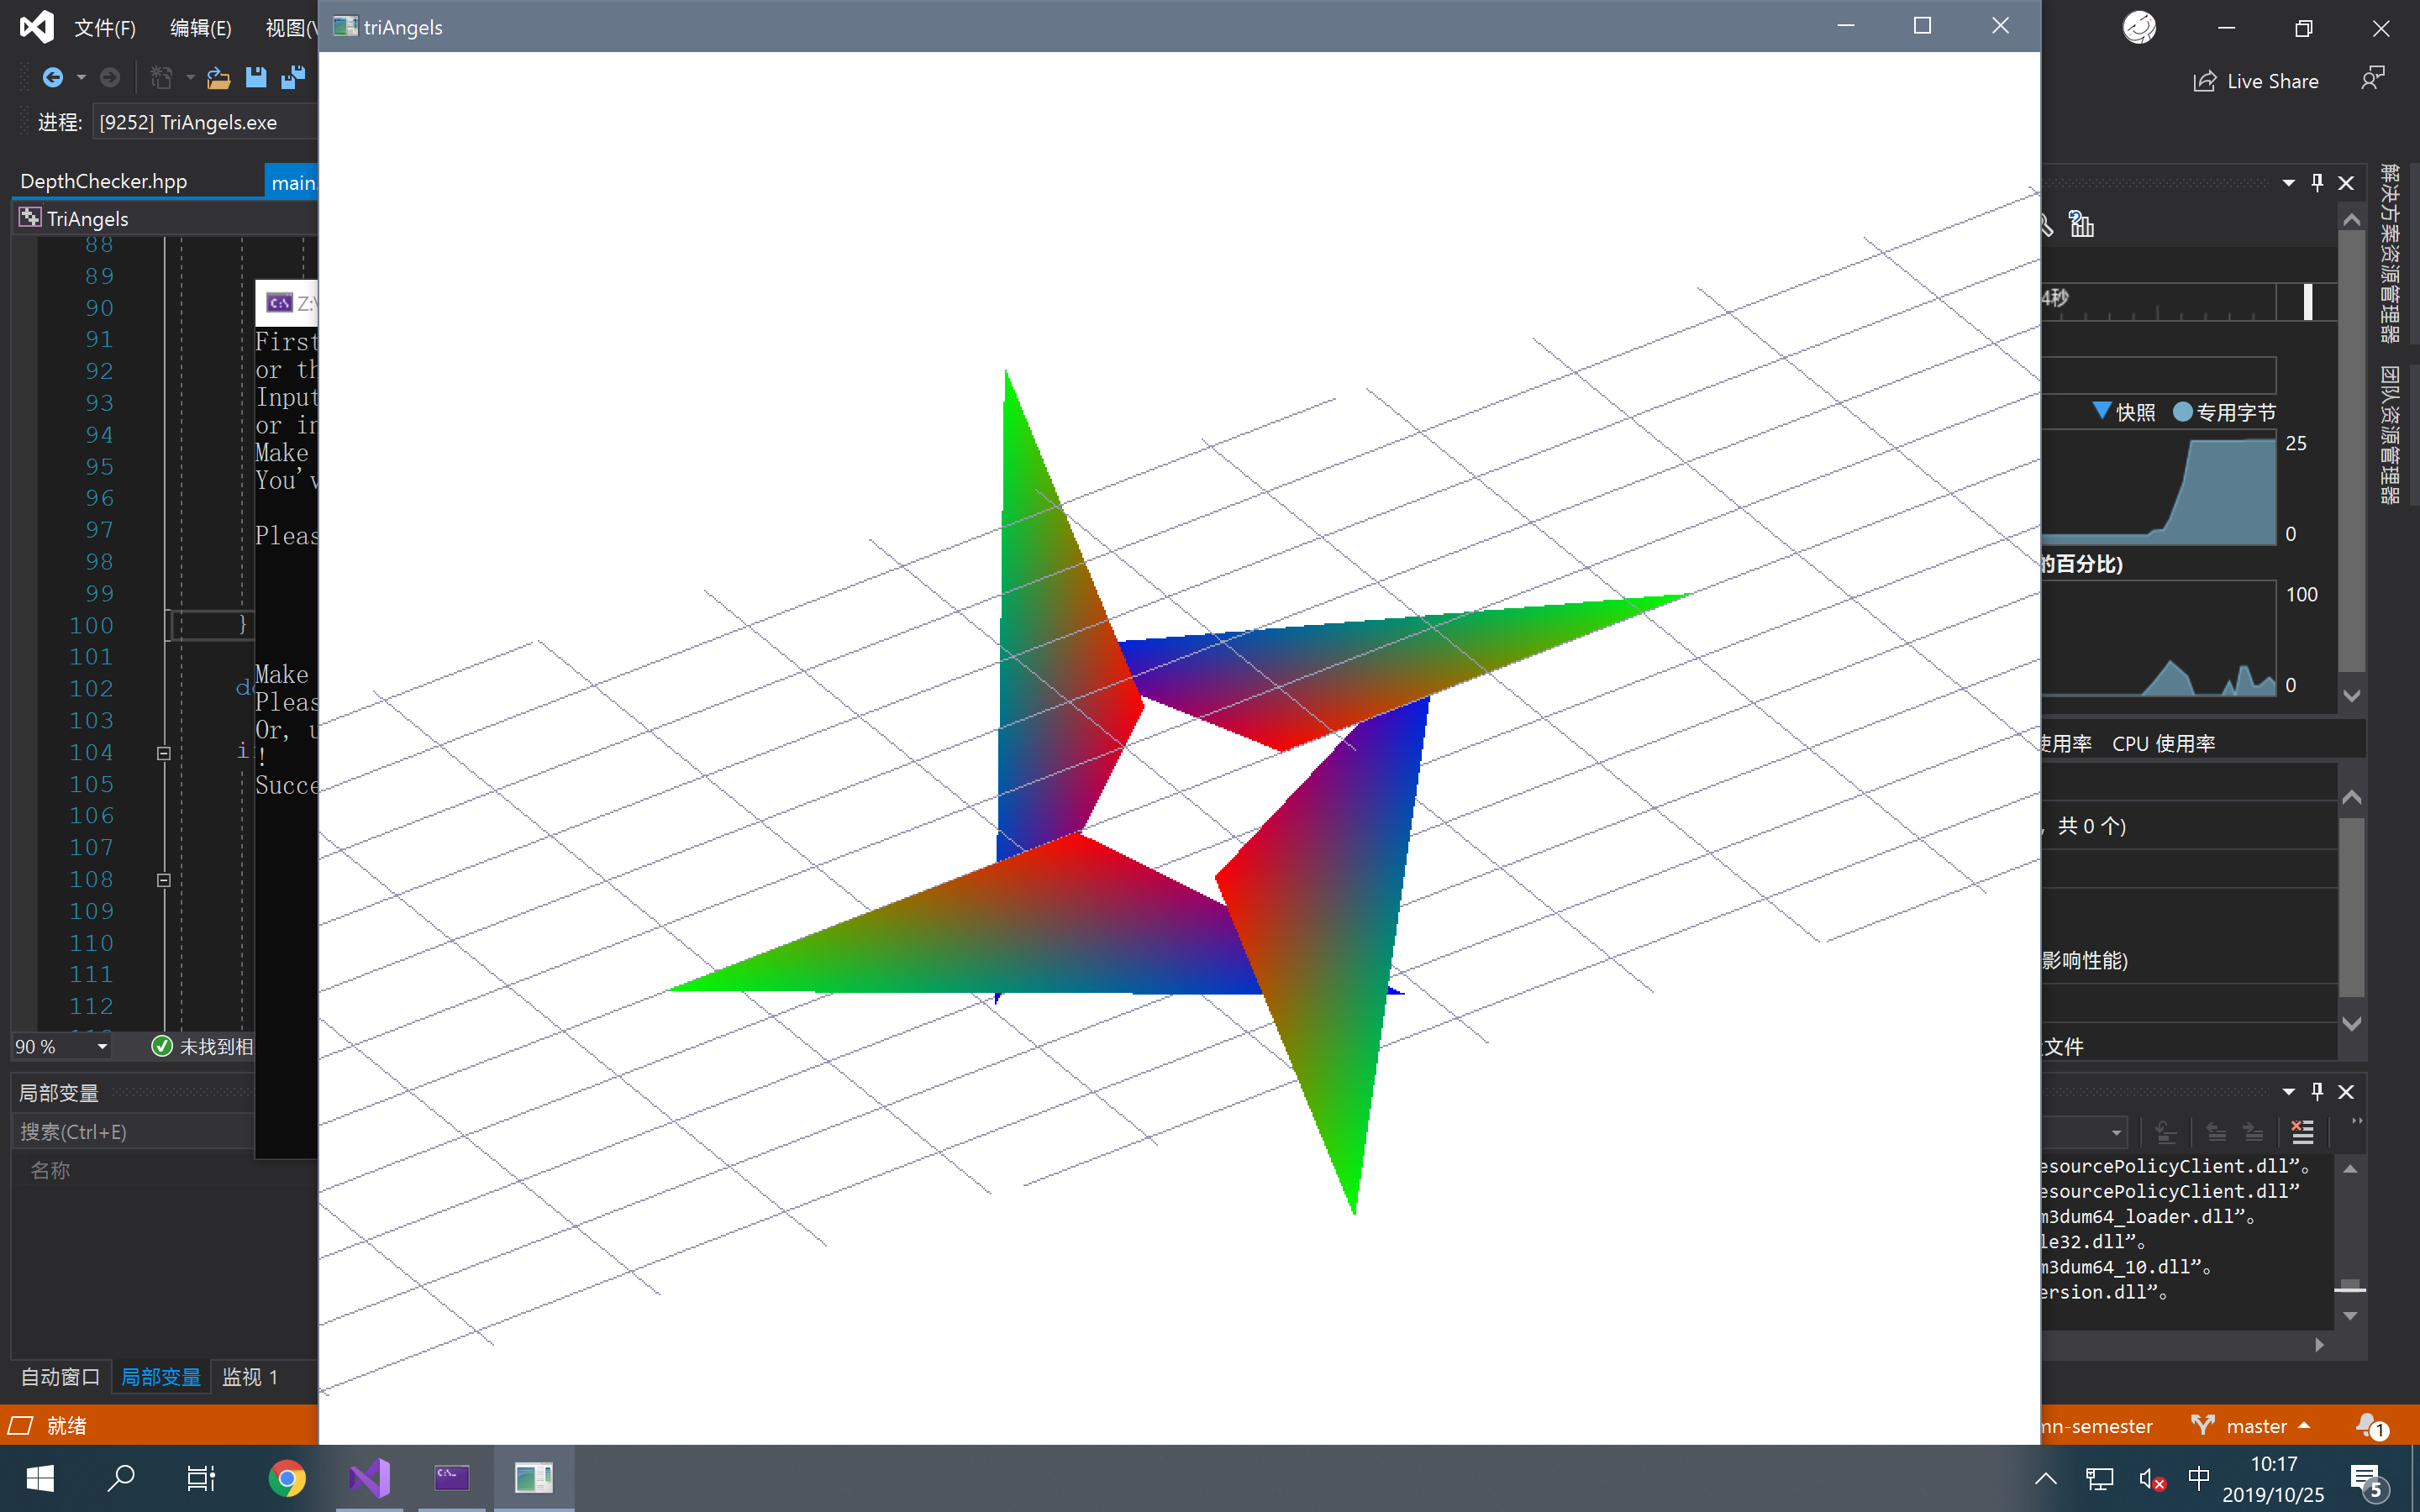
\includegraphics{/Users/yue/Documents/GitHub/2019-2020-autumn-semester/SE-344/submissions/ass2/screenshots/img.001.png}
\caption{}
\end{figure}

\begin{quote}
「\texttt{overlapping.tri}」的渲染结果,使用随附的深度检测算法
\end{quote}

\begin{figure}
\centering
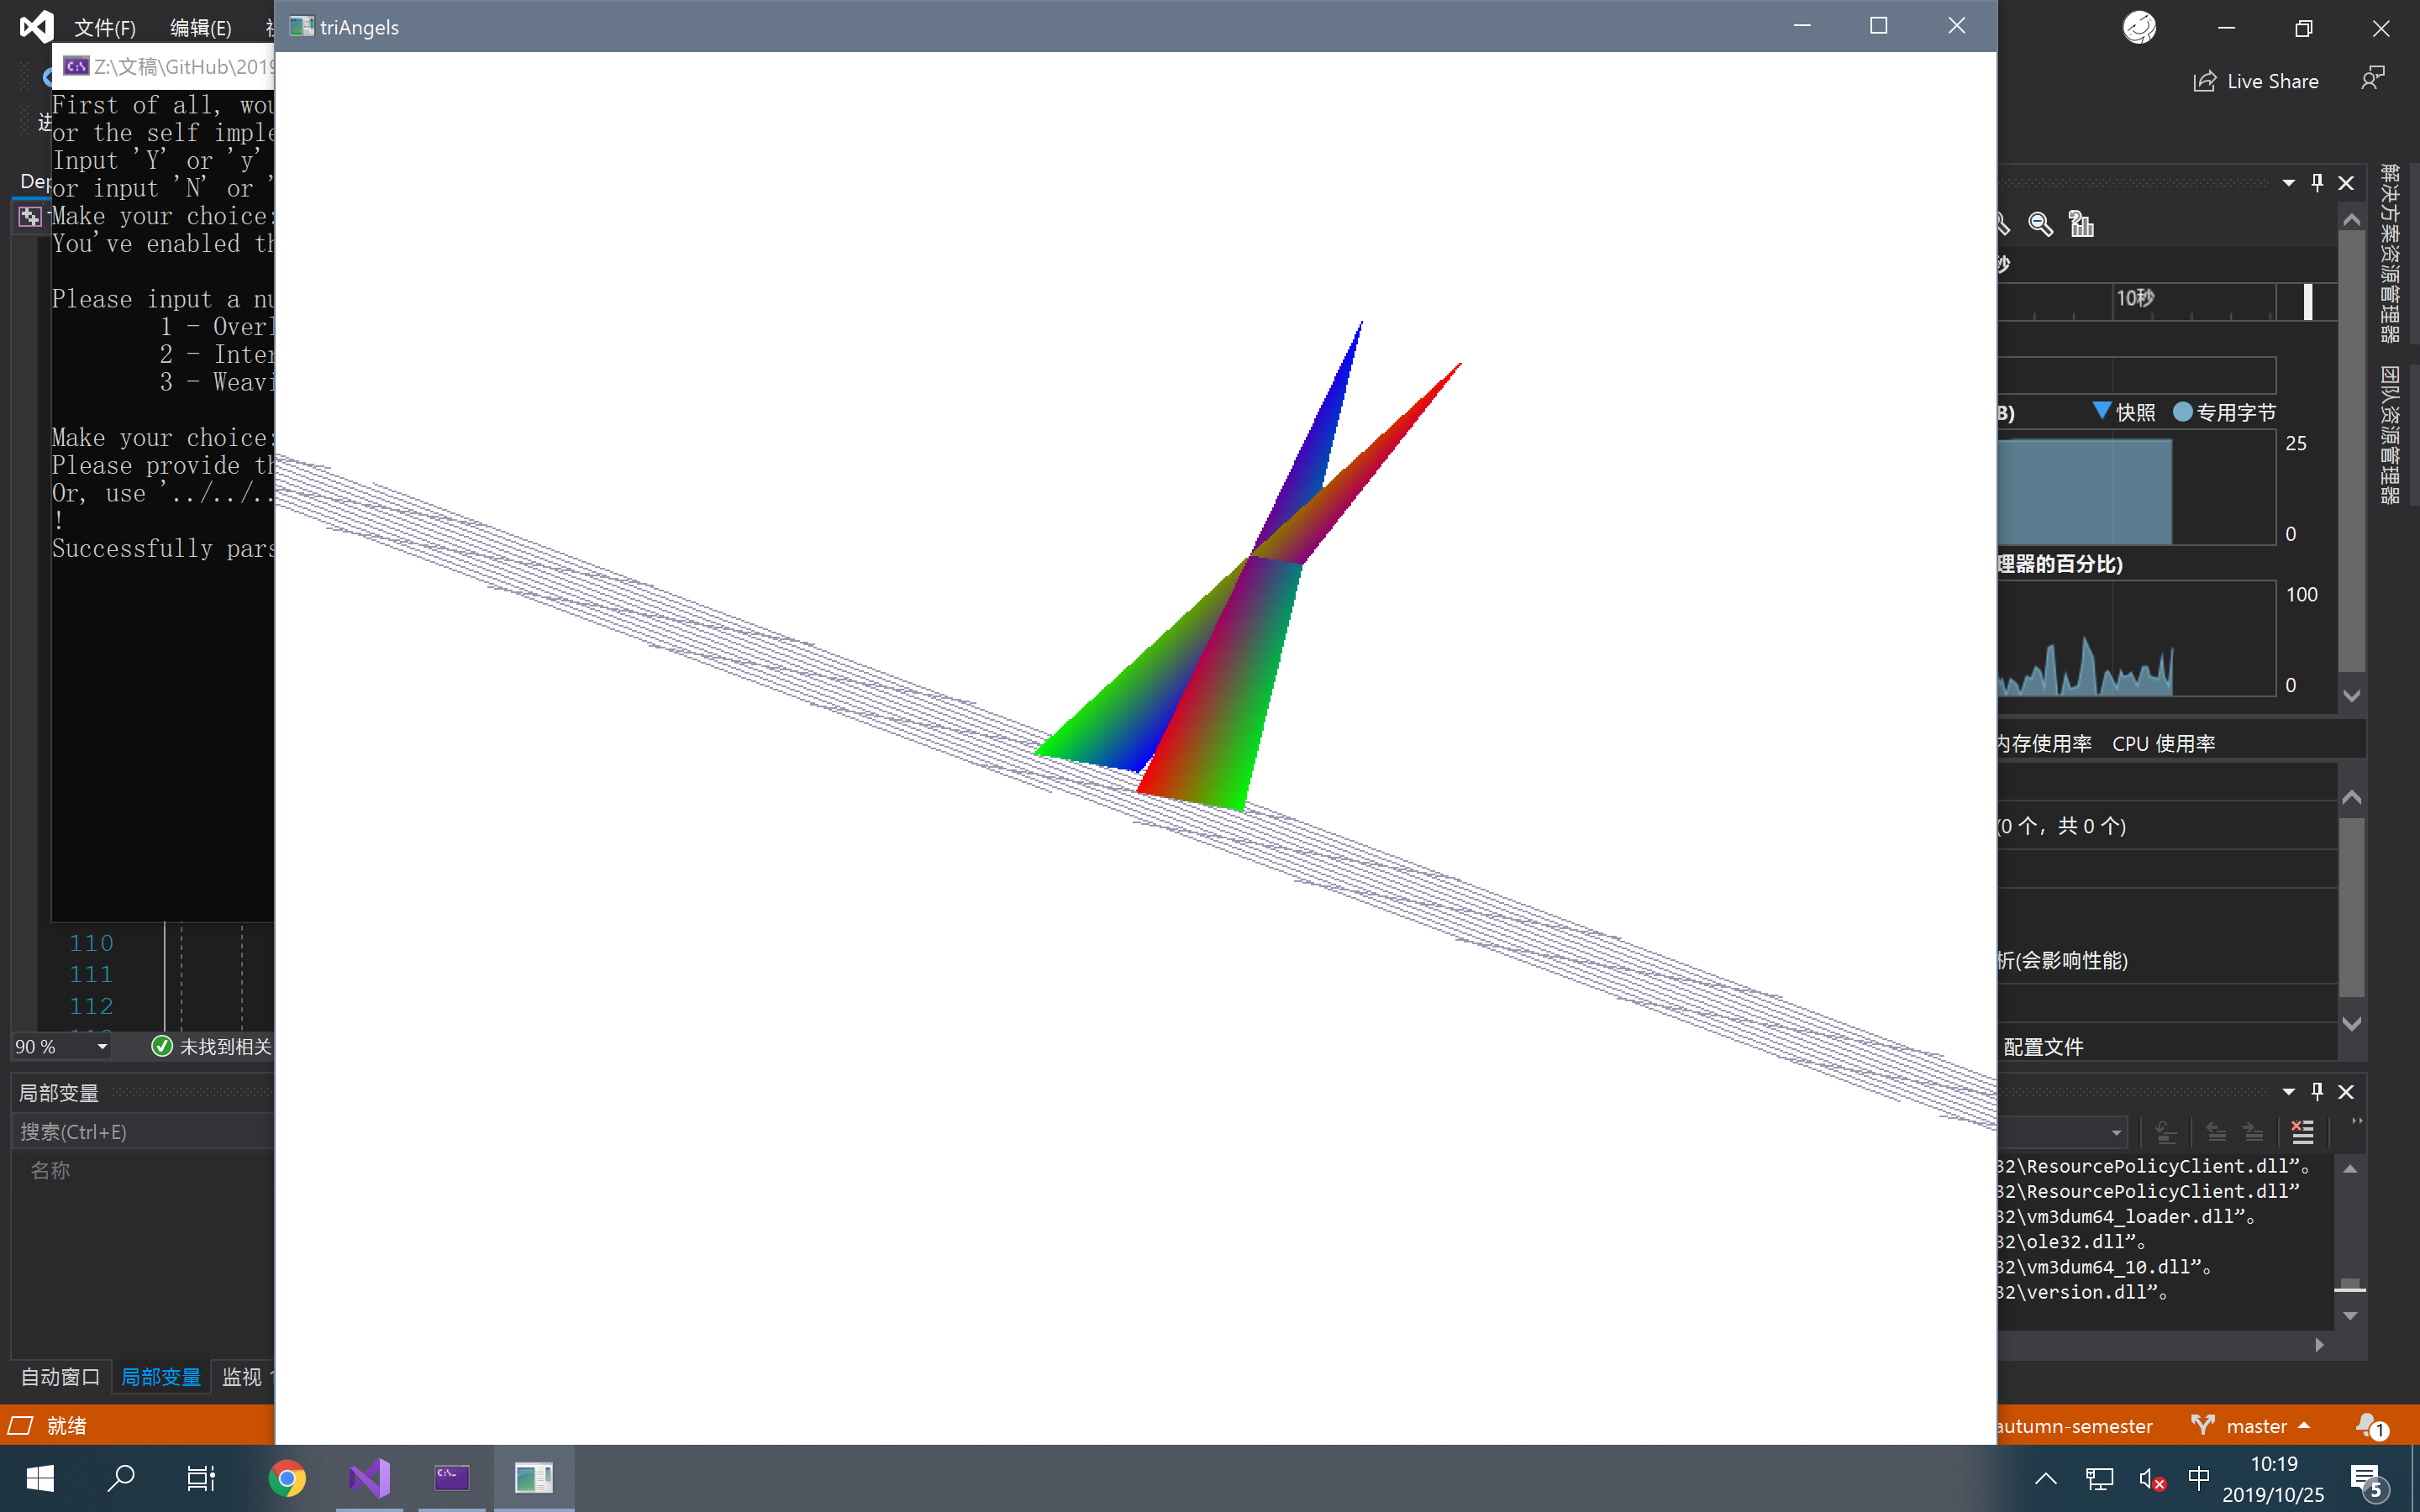
\includegraphics{/Users/yue/Documents/GitHub/2019-2020-autumn-semester/SE-344/submissions/ass2/screenshots/img.002.png}
\caption{}
\end{figure}

\begin{quote}
「\texttt{intersecting.tri}」的渲染结果,使用随附的深度检测算法
\end{quote}

\hypertarget{header-n86}{%
\paragraph{第四部分:扫描线算法}\label{header-n86}}

\hypertarget{header-n87}{%
\subparagraph{兼容修改}\label{header-n87}}

为了保证在实现扫描线算法的过程中,不要破坏上面已经完成的代码,这里新增了一个名为
\texttt{useDefaultDepthCheck}
的开关;程序运行起始会询问是否打开这一开关。

\hypertarget{header-n89}{%
\subparagraph{思路说明}\label{header-n89}}

为了简便起见,也因为图形较为简单,这里使用了最简单的思路:

\begin{enumerate}
\def\labelenumi{\arabic{enumi}.}
\item
  在 \(xOy\)
  平面内遍历所有点,判断其是否和三角形存在交点;映射完成后跳转到第 5
  步。
\item
  如果不存在交点,则忽略该点,回到第 1 步;
\item
  若存在唯一交点,则插值计算该交点的 \(z\) 坐标,并将 \((x, y, z)\)
  加入点映射表,回到第 1 步;
\item
  若存在多于 1
  个交点,则分别计算不同三角形的插值坐标,并比较采用其中最大的 \(z\)
  值,将其加入映射表;回到第 1 步;
\item
  从映射表中抽离出一个点集并返回给渲染器进行绘制。
\end{enumerate}

\hypertarget{header-n102}{%
\subparagraph{数学分析}\label{header-n102}}

这里存在两个数学问题:

一是如何判断与 \(z\) 轴平行的直线 \(x = x_0, y = y_0\) 是否穿过三角形;

二是如果穿过三角形,如何计算这条直线和三角形的交点坐标;

三是已知交点坐标,如何确定交点的 R、G、B 分量。

我们分别来进行分析。

相交判定

由于我们的渲染方向固定(沿着 \(z\)
轴向负方向观察),因此可以将三角形投影到 \(xOy\) 平面上进行计算。

于是问题可以抽象化为:已知平面 \(xOy\) 上四点
\(A\)、\(B\)、\(C\)、\(P\),判断点 P 是否在 \(A\)、\(B\)、\(C\)
构成的三角形内部。

这是一个简单的平面几何题。

要判断点是否在三角形内部,我们首先简化到判断点是否在一个方向向量的一侧。

而判断一个点是否在一个方向向量的一侧(左侧或右侧),我们可以采用差积(符号为
\(\times\))进行计算。

设已知的方向向量为 \(\overrightarrow{AB}\),要判断的点为
\(P\),则我们只需要判断向量 \(\overrightarrow{AB}\) 和
\(\overrightarrow{AP}\) 差积的符号即可。

当 \(P\) 在 \(\overrightarrow{AB}\)
左侧时,\(\overrightarrow{AB} \times \overrightarrow{AP}\)
应为正(根据右手螺旋法则);反之则在其右侧。

那么拓展到整个三角形,当点 \(P\) 同时在
\(\overrightarrow{AB}\)、\(\overrightarrow{BC}\)、\(\overrightarrow{CA}\)
的同侧时,即可判断其在三角形内部了。

\begin{quote}
\texttt{DepthChecker.hpp} 中的 \texttt{inTriangle} 函数实现了上述算法。
\end{quote}

交点计算

根据立体几何知识,不共线三点能确定一个平面。因此我们首先根据公式组

\[\left\{
\begin{aligned}
a & = & (p_{2_y} - p_{1_y}) \times (p_{3_z} - p_{1_z}) - (p_{2_z} - p_{1_z}) \times (p_{3_y} - p_{1_y}) \\
b & = & (p_{2_z} - p_{1_z}) \times (p_{3_x} - p_{1_x}) - (p_{2_x} - p_{1_x}) \times (p_{3_z} - p_{1_z}) \\
c & = & (p_{2_x} - p_{1_x}) \times (p_{3_y} - p_{1_y}) - (p_{2_y} - p_{1_y}) \times (p_{3_x} - p_{1_x}) \\
d & = &  - (a \times p_{1_x} + b \times p_{1_y} + c \times p_{1_z})
\end{aligned}
\right.\]

解出三点确定的平面公式 \(ax + by + cx + d = 0\)。

之后,我们将已知的射线 \(x = x_0, y = y_0\) 代入即可求出交点
\((x_0, y_0, z_0)\)。

\begin{quote}
\texttt{Triangle.hpp} 中的成员方法 \texttt{getPanelEquation}
实现了上述算法。
\end{quote}

颜色确定

这是一个比较麻烦的算法,主要原因是为了保证效果和原始图像的统一性,必须使用和原图相似的重心差值算法来进行颜色填充。

考虑到三角形是个平面图形,投影不会改变其插值性质;因此直接将其向观察面
\(xOy\) 上投影并计算颜色。

而计算颜色分量,本质上是计算三角形三个顶点的颜色决定权重;即每个点对于目标点具有多大的影响力。

重心坐标算法的思路是:\(A\) 点对于 \(P\) 点的权重,等于三角形 \(BCP\)
的面积在大三角形 \(ABC\) 的面积中所占的比例。

这样的计算方法可以保证在端点处的颜色分配正确性,以及始终能保证归一:三角形的总面积分成三份,总能保证其和为整个三角形的面积。

\begin{quote}
利用了 Mathematica 对各点权值进行计算。工作簿文件参见
\texttt{/ass2/math/color\_setting.nb}。
\end{quote}

实际公式如下:

\[\left\{
\begin{aligned}
u & = & -\frac{(P.y-\text{P1}.y) (\text{P1}.x-\text{P3}.x)-(P.x-\text{P1}.x) (\text{P1}.y-\text{P3}.y)}{(\text{P1}.y-\text{P2}.y) (\text{P1}.x-\text{P3}.x)-(\text{P1}.x-\text{P2}.x) (\text{P1}.y-\text{P3}.y)} \\

v & = & -\frac{-P.y \text{P1}.x+P.x \text{P1}.y+P.y \text{P2}.x-P.x \text{P2}.y+\text{P1}.x \text{P2}.y-\text{P1}.y \text{P2}.x}{\text{P1}.y \text{P2}.x-\text{P1}.x \text{P2}.y-\text{P1}.y \text{P3}.x+\text{P1}.x \text{P3}.y-\text{P2}.x \text{P3}.y+\text{P2}.y \text{P3}.x}

\end{aligned}
\right.\]

其中,\(u\) 对应 \(P1\) 的权值;\(v\) 对应 \(P2\) 的权值;而 \(P3\)
的权值可利用 \(1 - u - v\) 计算得出。

\begin{quote}
\texttt{DepthChecker.hpp} 的 \texttt{analyse} 方法中实现了颜色确定算法。
\end{quote}

\hypertarget{header-n139}{%
\subparagraph{栅格渲染}\label{header-n139}}

使用 \texttt{DepthChecker} 类即可实现栅格化的三角形渲染。

\texttt{onRender} 方法被调用时,会首先检测 \texttt{useDefaultDepthCheck}
开关是否被打开。

如果该开关被关闭,则会关闭默认的深度检测,并且先使用
\texttt{DepthChecker} 来栅格化得到的三角形。

随后,使用 \texttt{glBegin(GL\_POINTS)} 方法来逐个绘制二维像素点。

\hypertarget{header-n144}{%
\subparagraph{观察结果}\label{header-n144}}

\begin{figure}
\centering
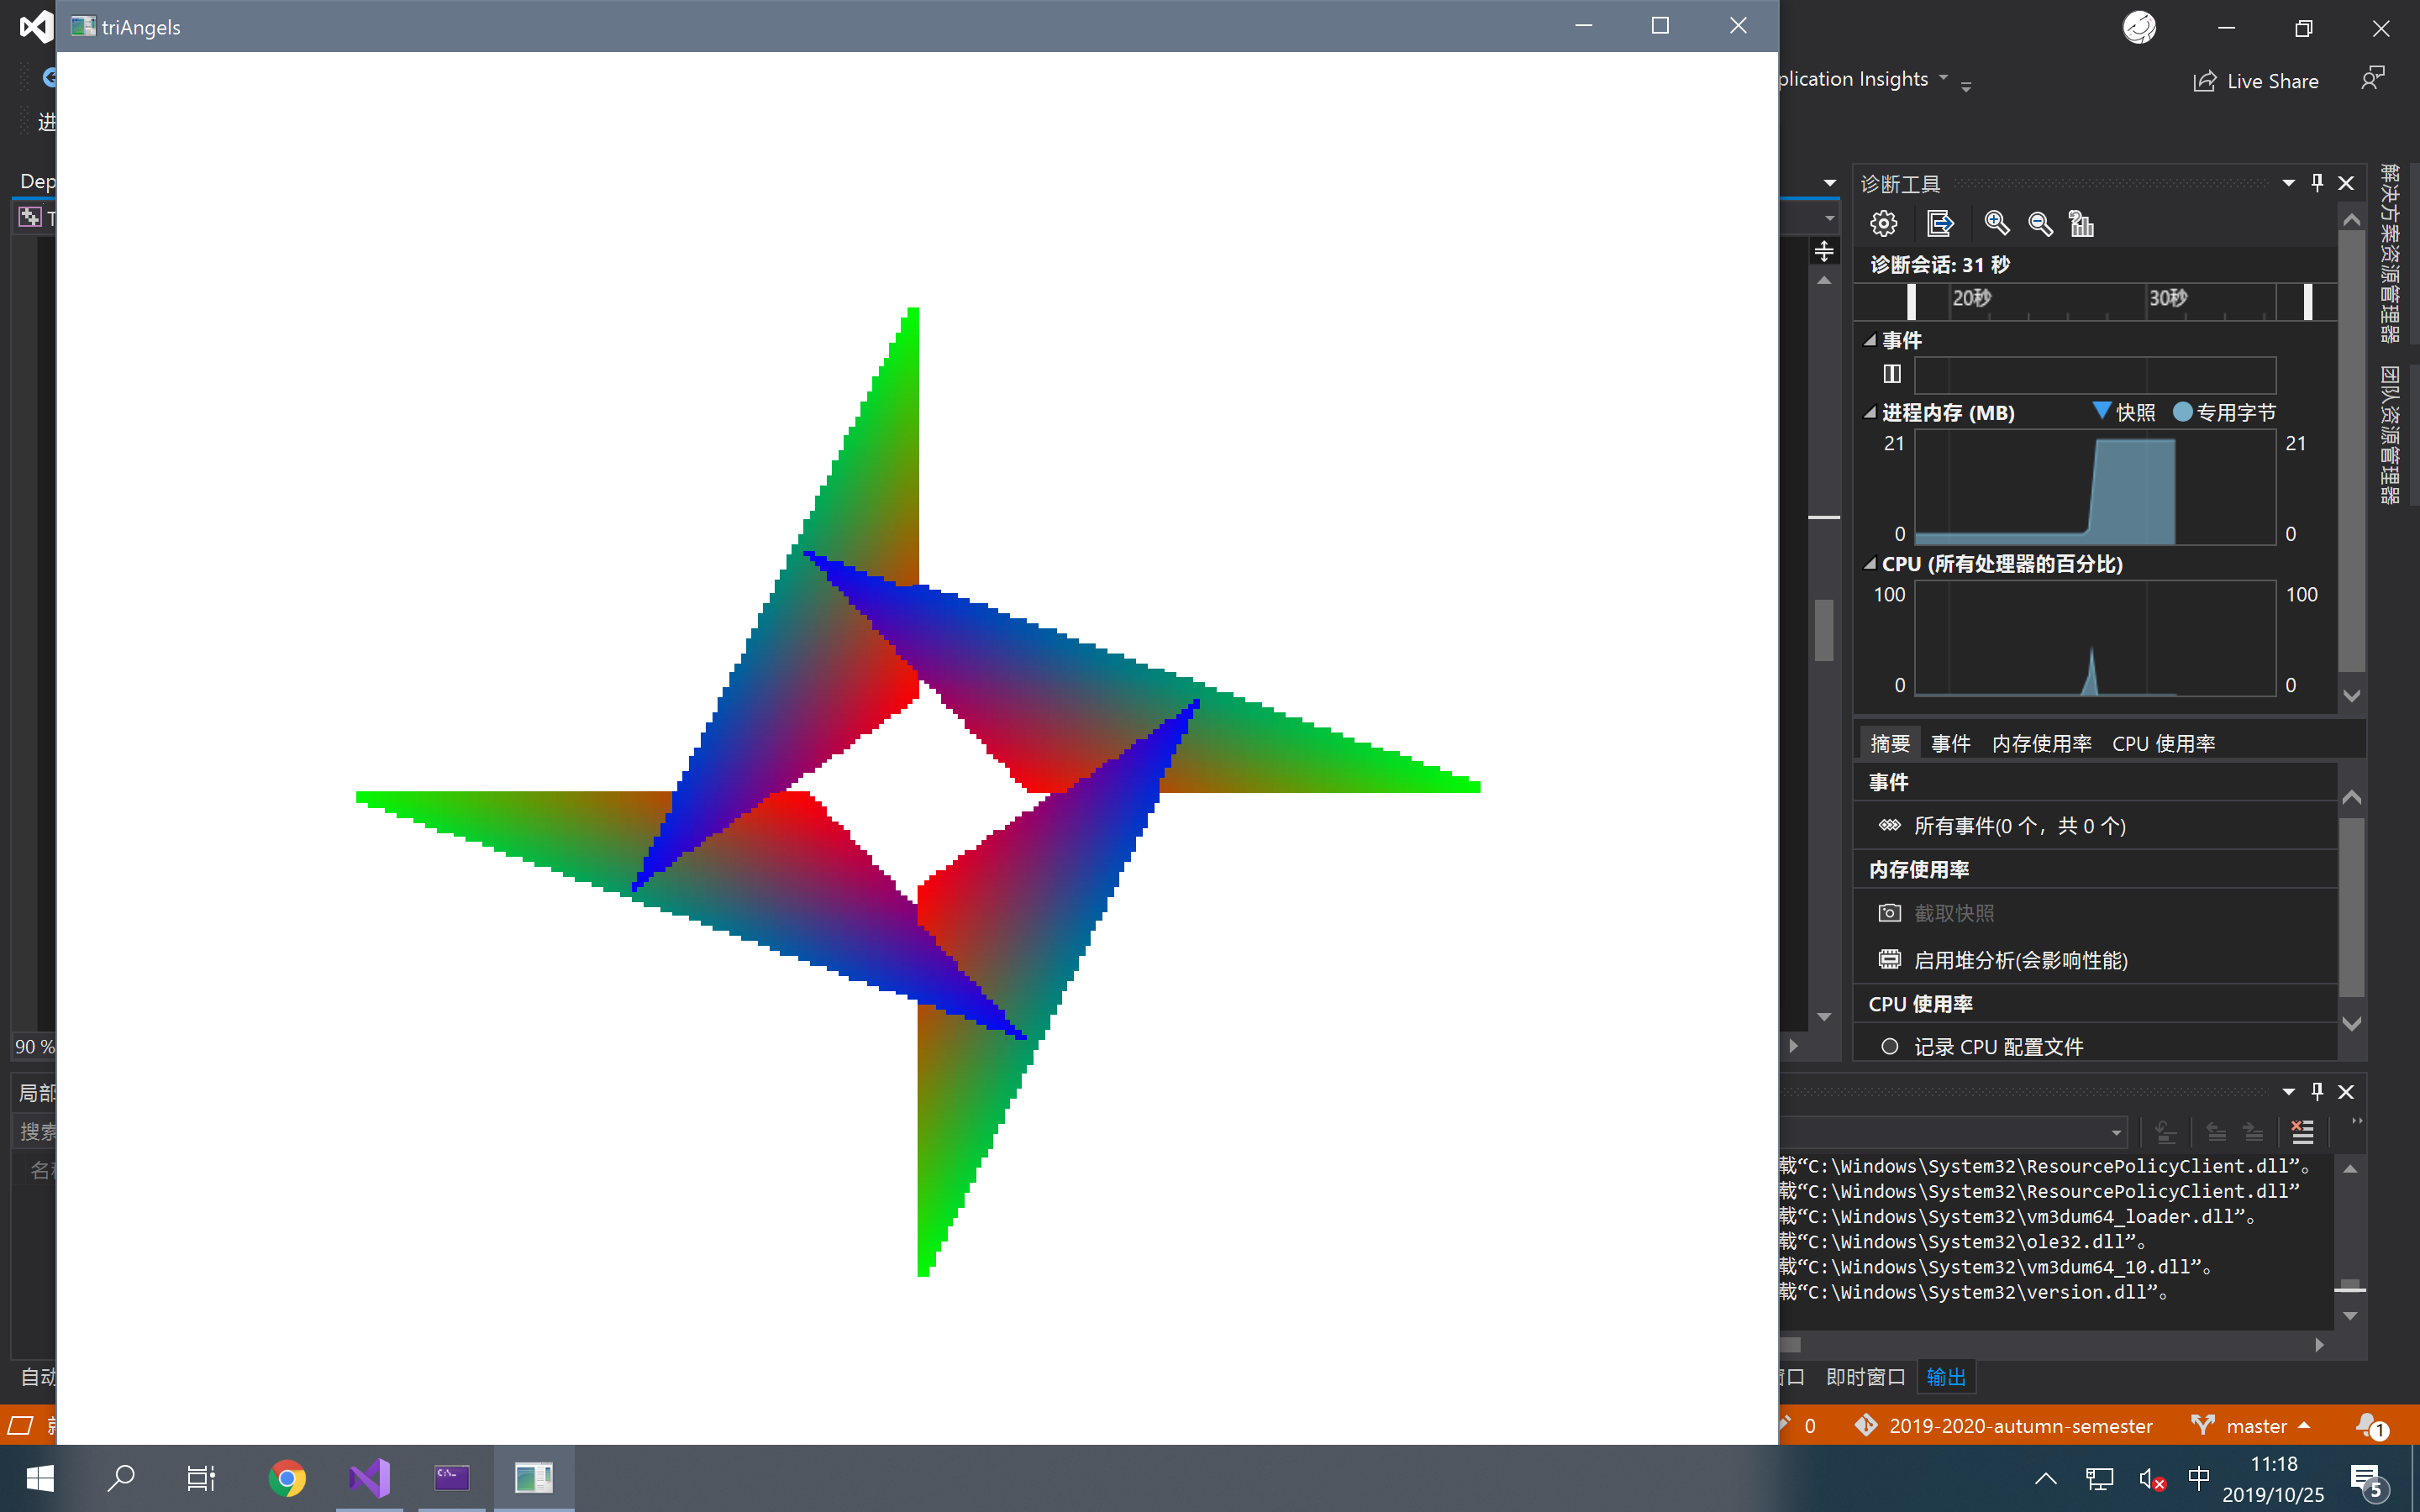
\includegraphics{/Users/yue/Documents/GitHub/2019-2020-autumn-semester/SE-344/submissions/ass2/screenshots/img.003.png}
\caption{}
\end{figure}

\begin{quote}
「\texttt{overlapping.tri}」的渲染结果,使用自定义的扫描线算法
\end{quote}

\begin{figure}
\centering
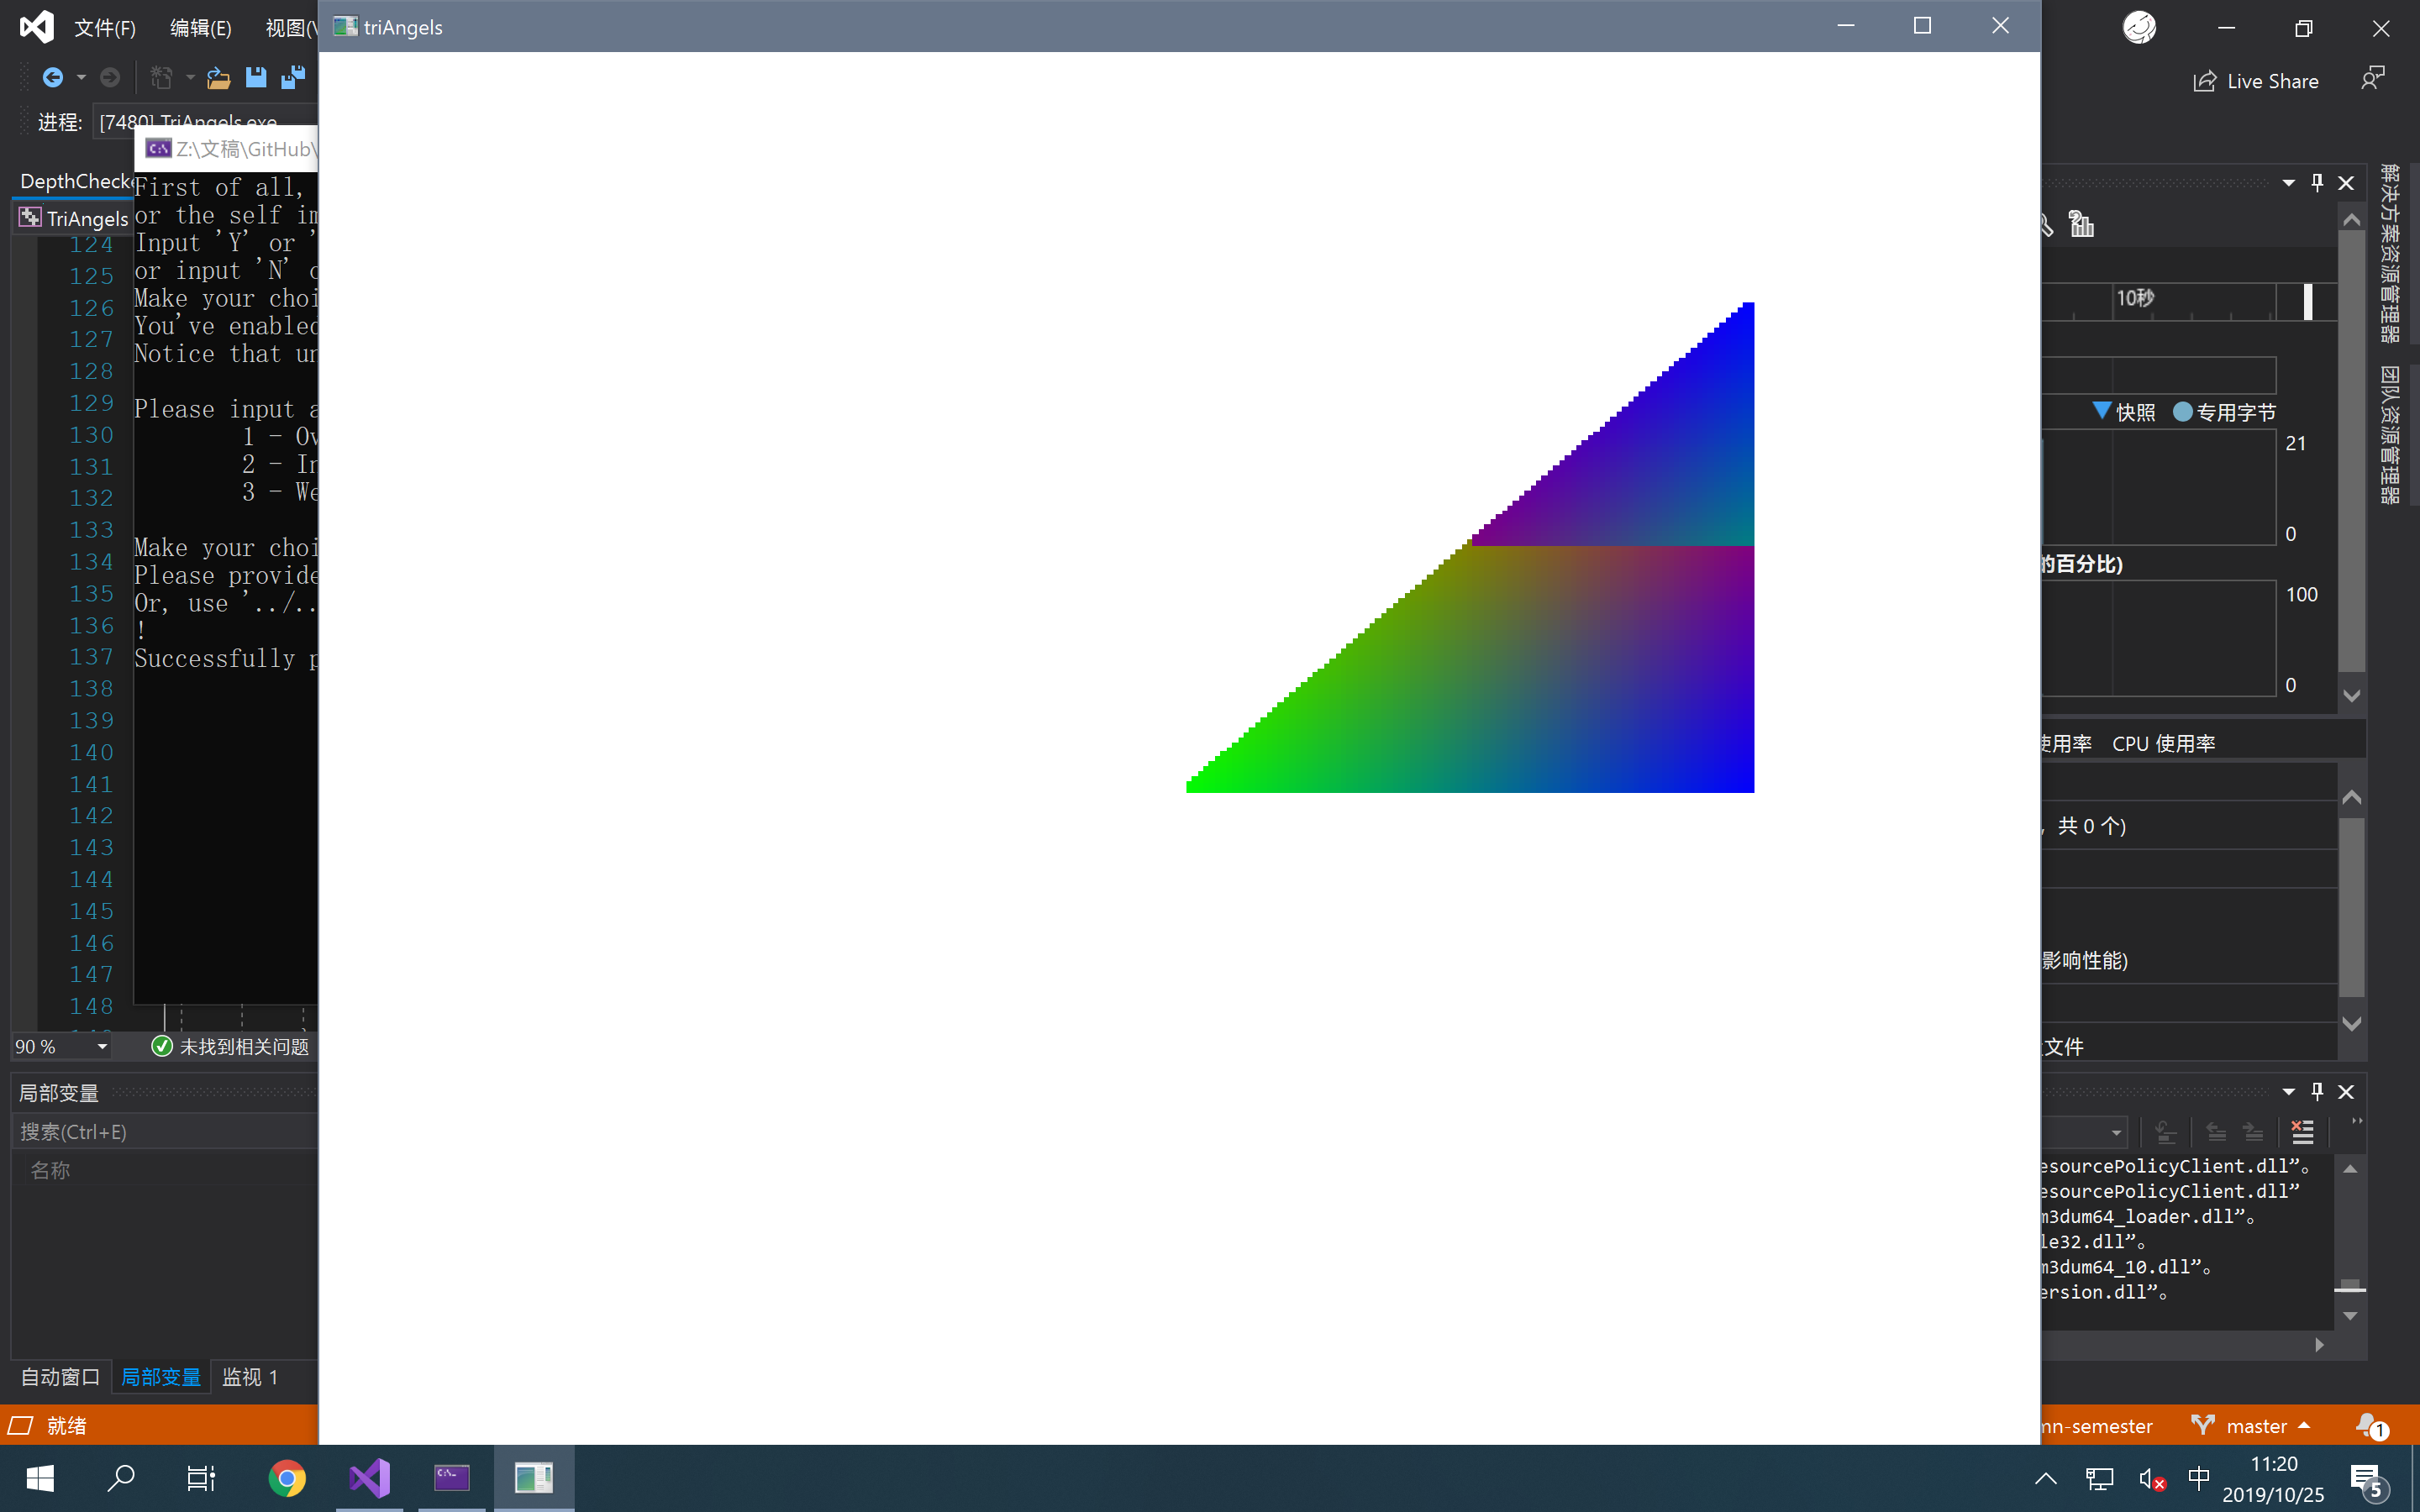
\includegraphics{/Users/yue/Documents/GitHub/2019-2020-autumn-semester/SE-344/submissions/ass2/screenshots/img.004.png}
\caption{}
\end{figure}

\begin{quote}
「\texttt{intersecting.tri}」的渲染结果,使用自定义的扫描线算法
\end{quote}

\begin{quote}
⚠️
留意到由于视角问题,两个三角形略有重合。但是从三角形中点连线的颜色突变可以看出
Intersecting 效果。
\end{quote}

\hypertarget{header-n153}{%
\paragraph{第四又半部分:视角调整}\label{header-n153}}

我们可以看到在自定义的扫描线算法中,正面看起来两个三角形重合了。

为了解决这个问题,我们在 \texttt{Triangle} 类中增加一个旋转方法。

算法的思路很简单:绕着 \(y\) 轴旋转 \(\theta\) 角只需要用
\(x = x\cos\theta \times z\sin\theta\) 计算即可。

绕着其他轴的计算结果类比得出。

旋转之后,\texttt{intersecting.tri} 的渲染结果如下:

\begin{figure}
\centering
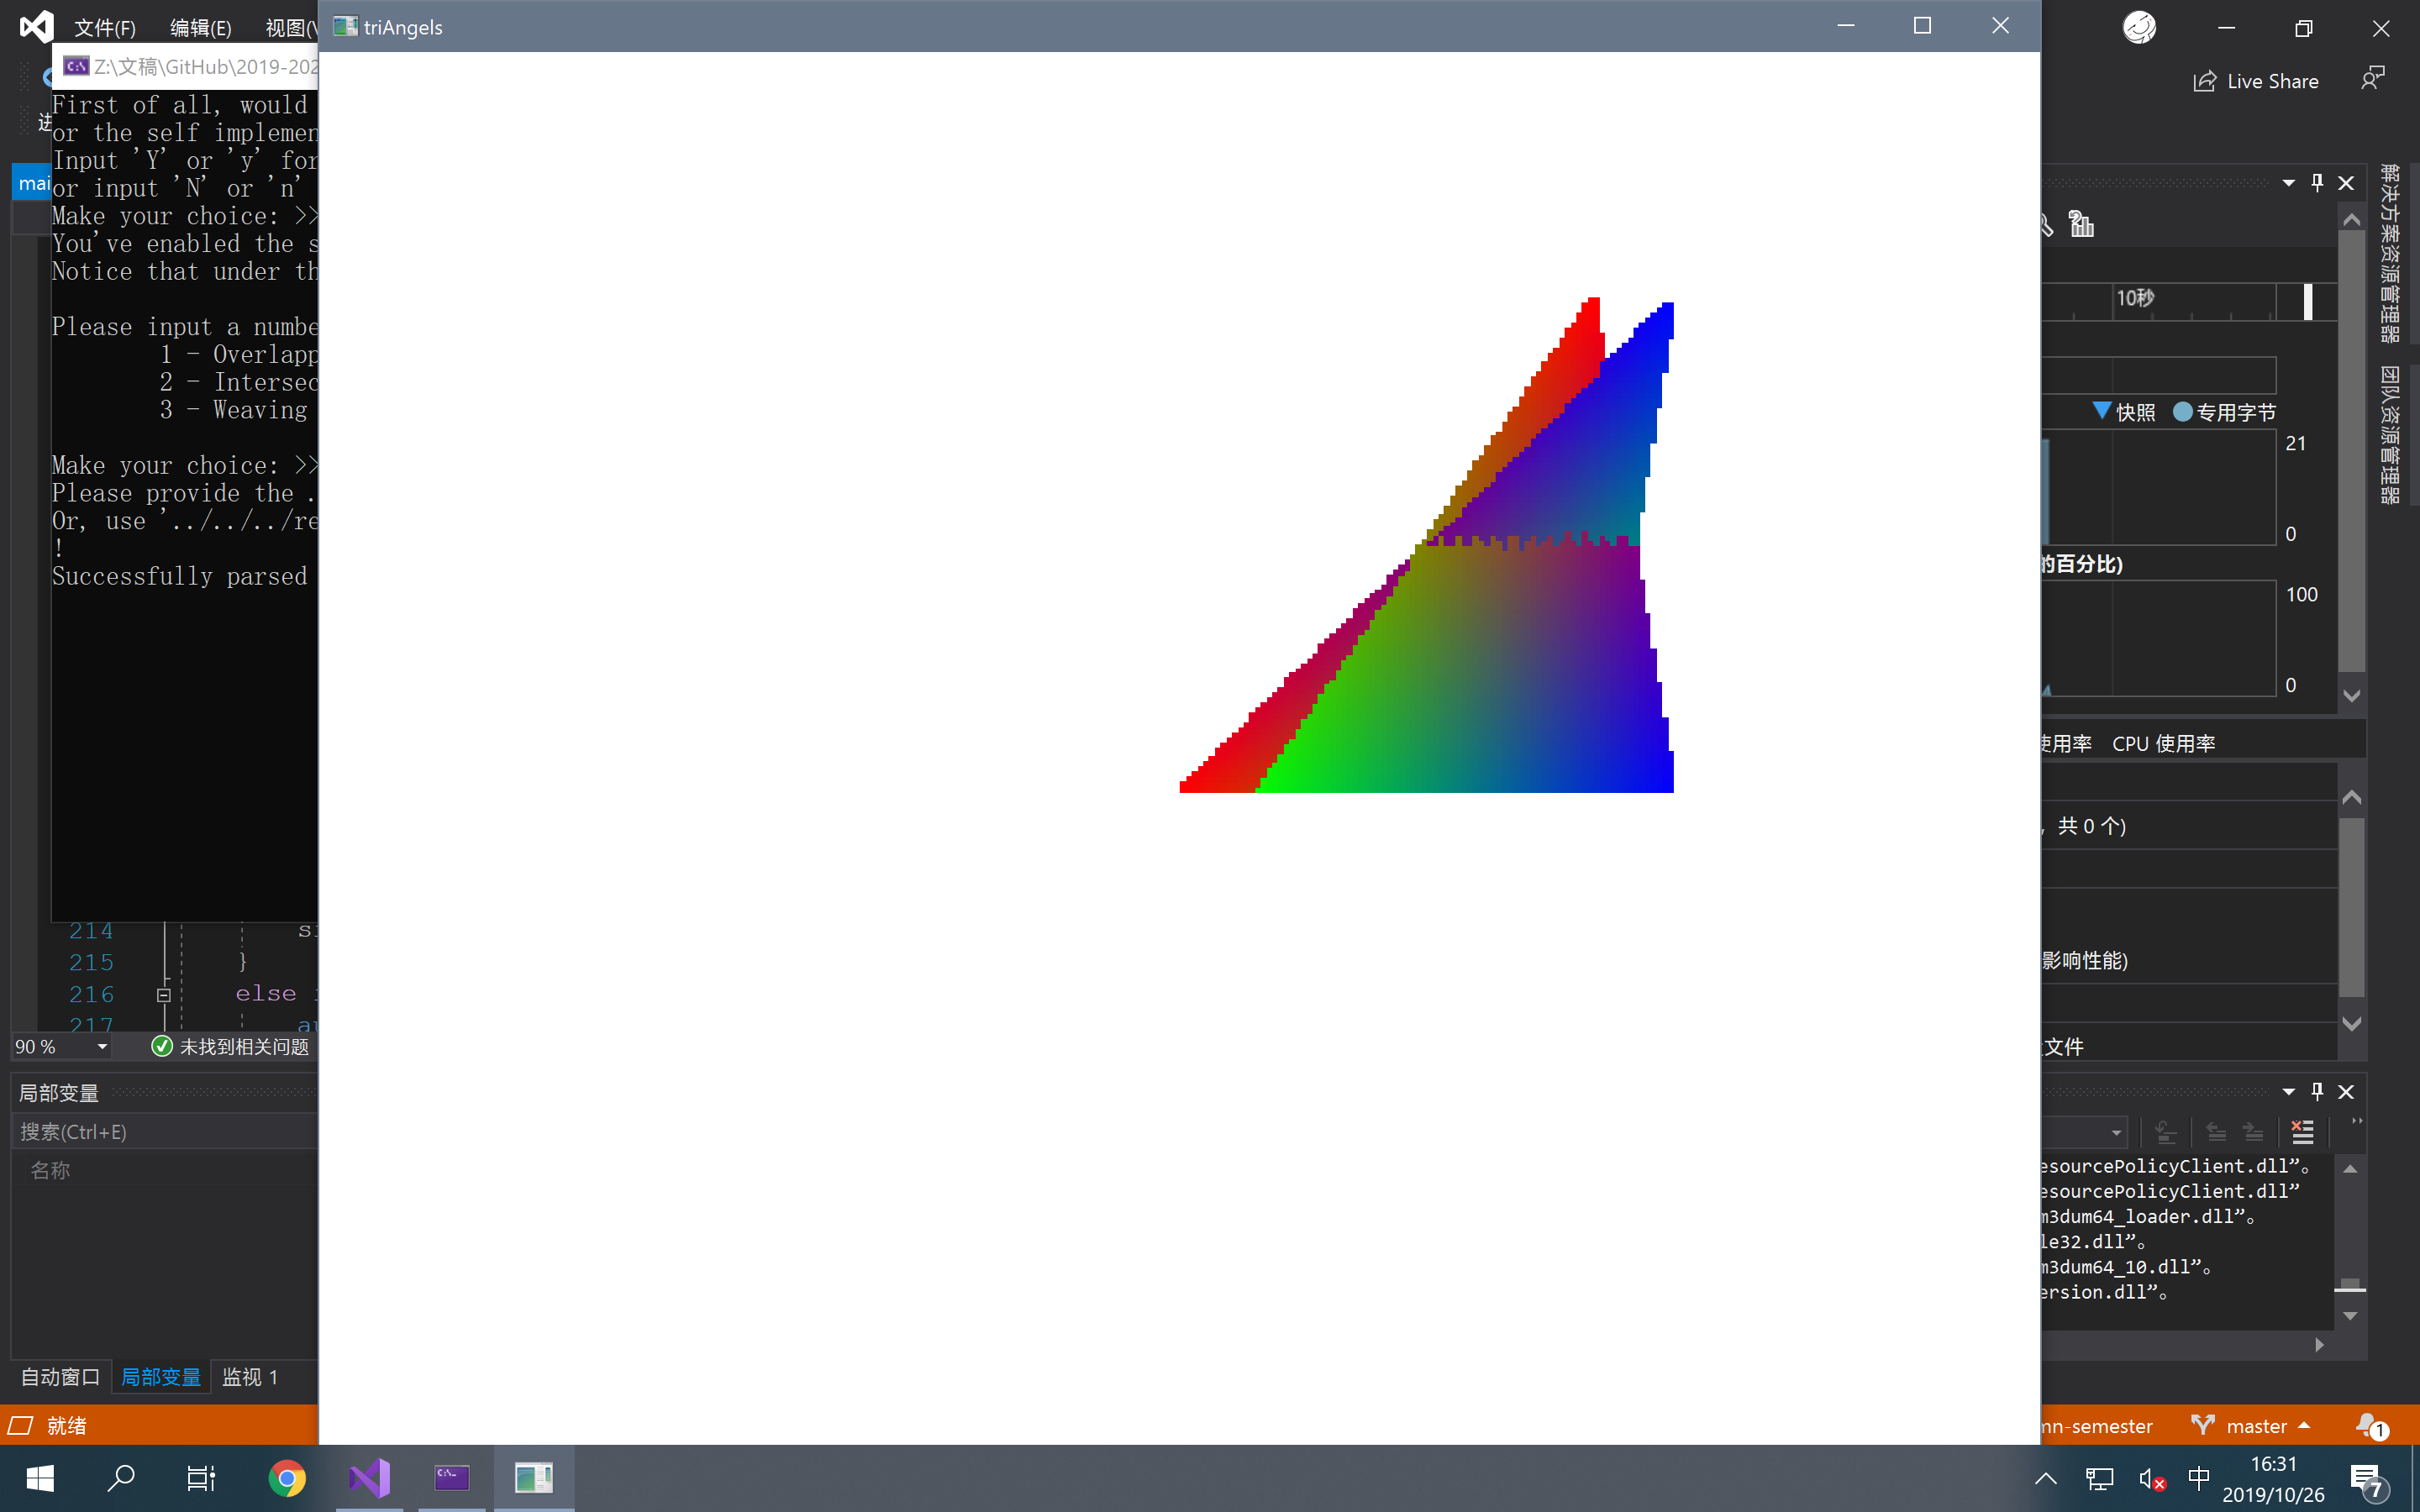
\includegraphics{/Users/yue/Documents/GitHub/2019-2020-autumn-semester/SE-344/submissions/ass2/screenshots/img.007.png}
\caption{}
\end{figure}

\begin{quote}
经旋转矫正后「\texttt{intersecting.tri}」的渲染结果,使用自定义的扫描线算法
\end{quote}

\hypertarget{header-n162}{%
\paragraph{第五部分:矩形编织}\label{header-n162}}

此部分相对于上面的算法没有特别之处。为了实现编织效果,这里采用的方式是模拟真实世界中的编织方式,令水平方向的条带始终维持在
\(xOy\) 平面上(即 \(z = 0\)),而令竖直方向的条带深度在 \(-1\) 和 \(1\)
之间摇摆,以实现类似于实际的编织效果。

\hypertarget{header-n164}{%
\subparagraph{程序结构}\label{header-n164}}

相关文件包括 \texttt{Weaving.hpp},其中的 \texttt{Weaving}
类可以生成实现矩形编织效果的三角形数组。

其主要逻辑为在一个 for
循环内反复生成三角形所构成的四边形,连接成条带状。

为了体现渲染器的普适性,将不对上面的渲染算法做任何更改。

\hypertarget{header-n168}{%
\subparagraph{优化效能}\label{header-n168}}

由于这里的所有连续条带都是单色的(不存在颜色渐变问题),因此在栅格化方法内提供一个单色模式,在此时不去计算颜色插值,而直接采用提供的单色来提高效率。

\hypertarget{header-n170}{%
\subparagraph{观察结果}\label{header-n170}}

\begin{figure}
\centering
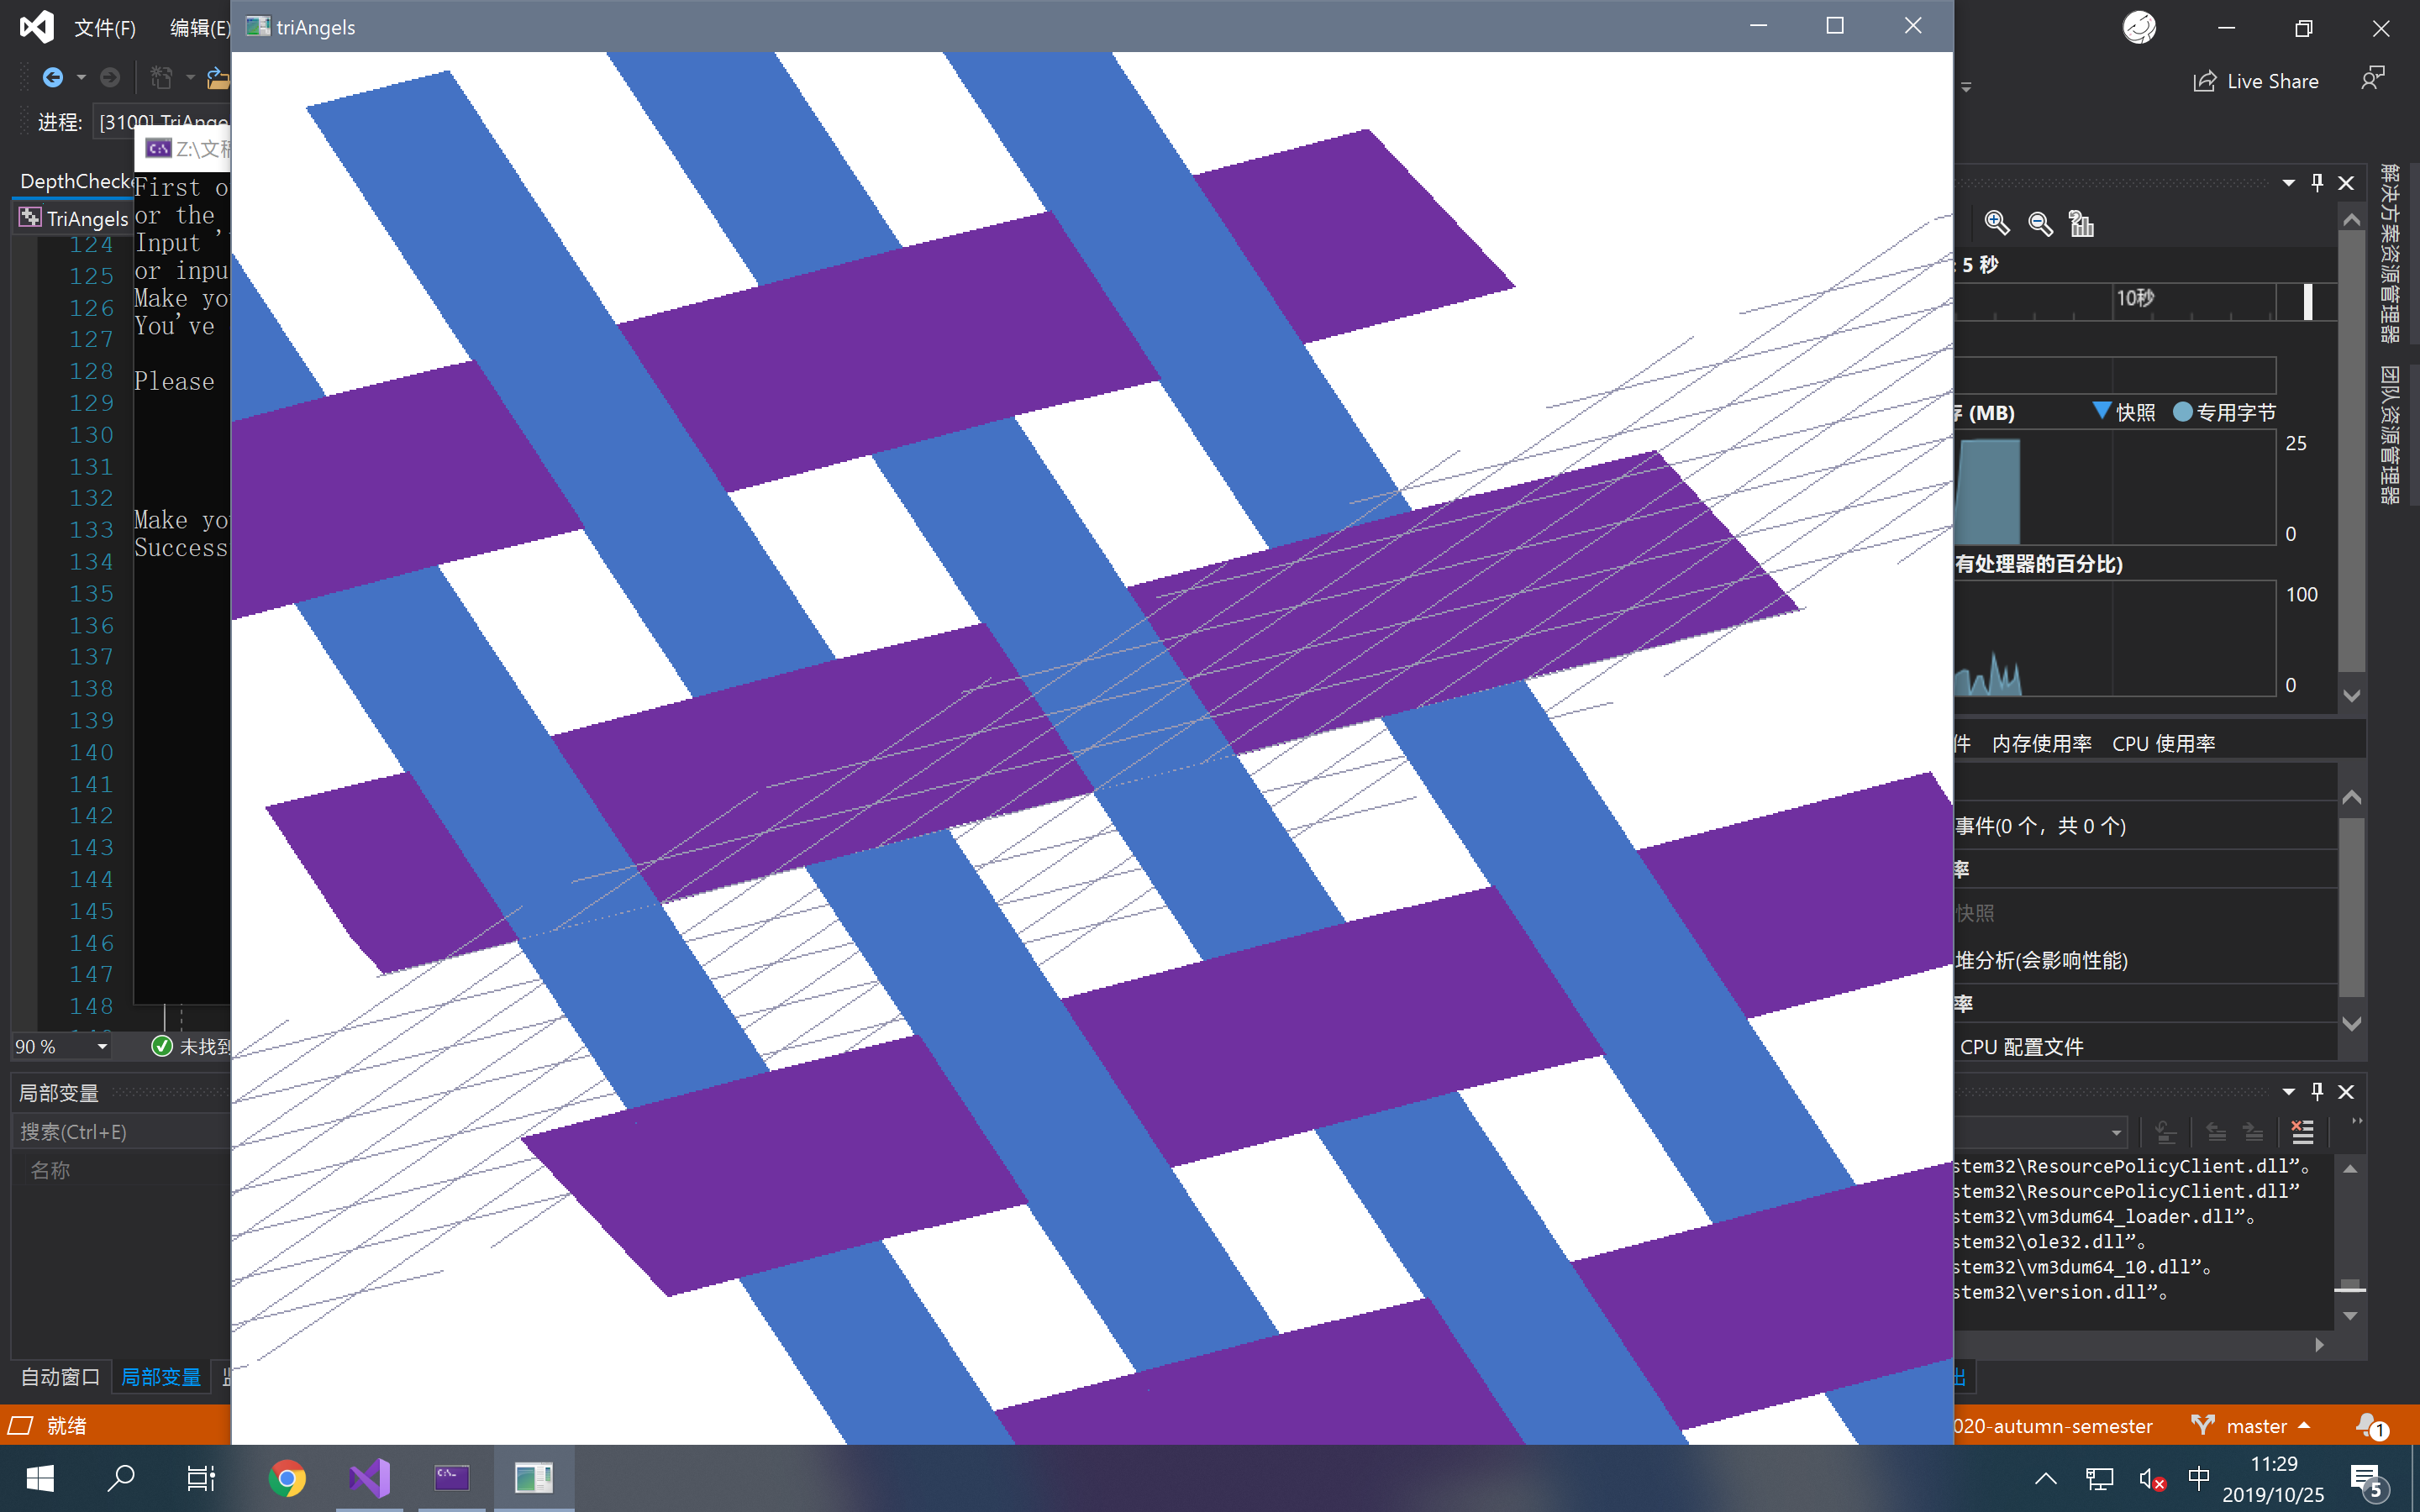
\includegraphics{/Users/yue/Documents/GitHub/2019-2020-autumn-semester/SE-344/submissions/ass2/screenshots/img.005.png}
\caption{}
\end{figure}

\begin{quote}
矩形编织效果,使用随附的深度检测算法
\end{quote}

\begin{figure}
\centering
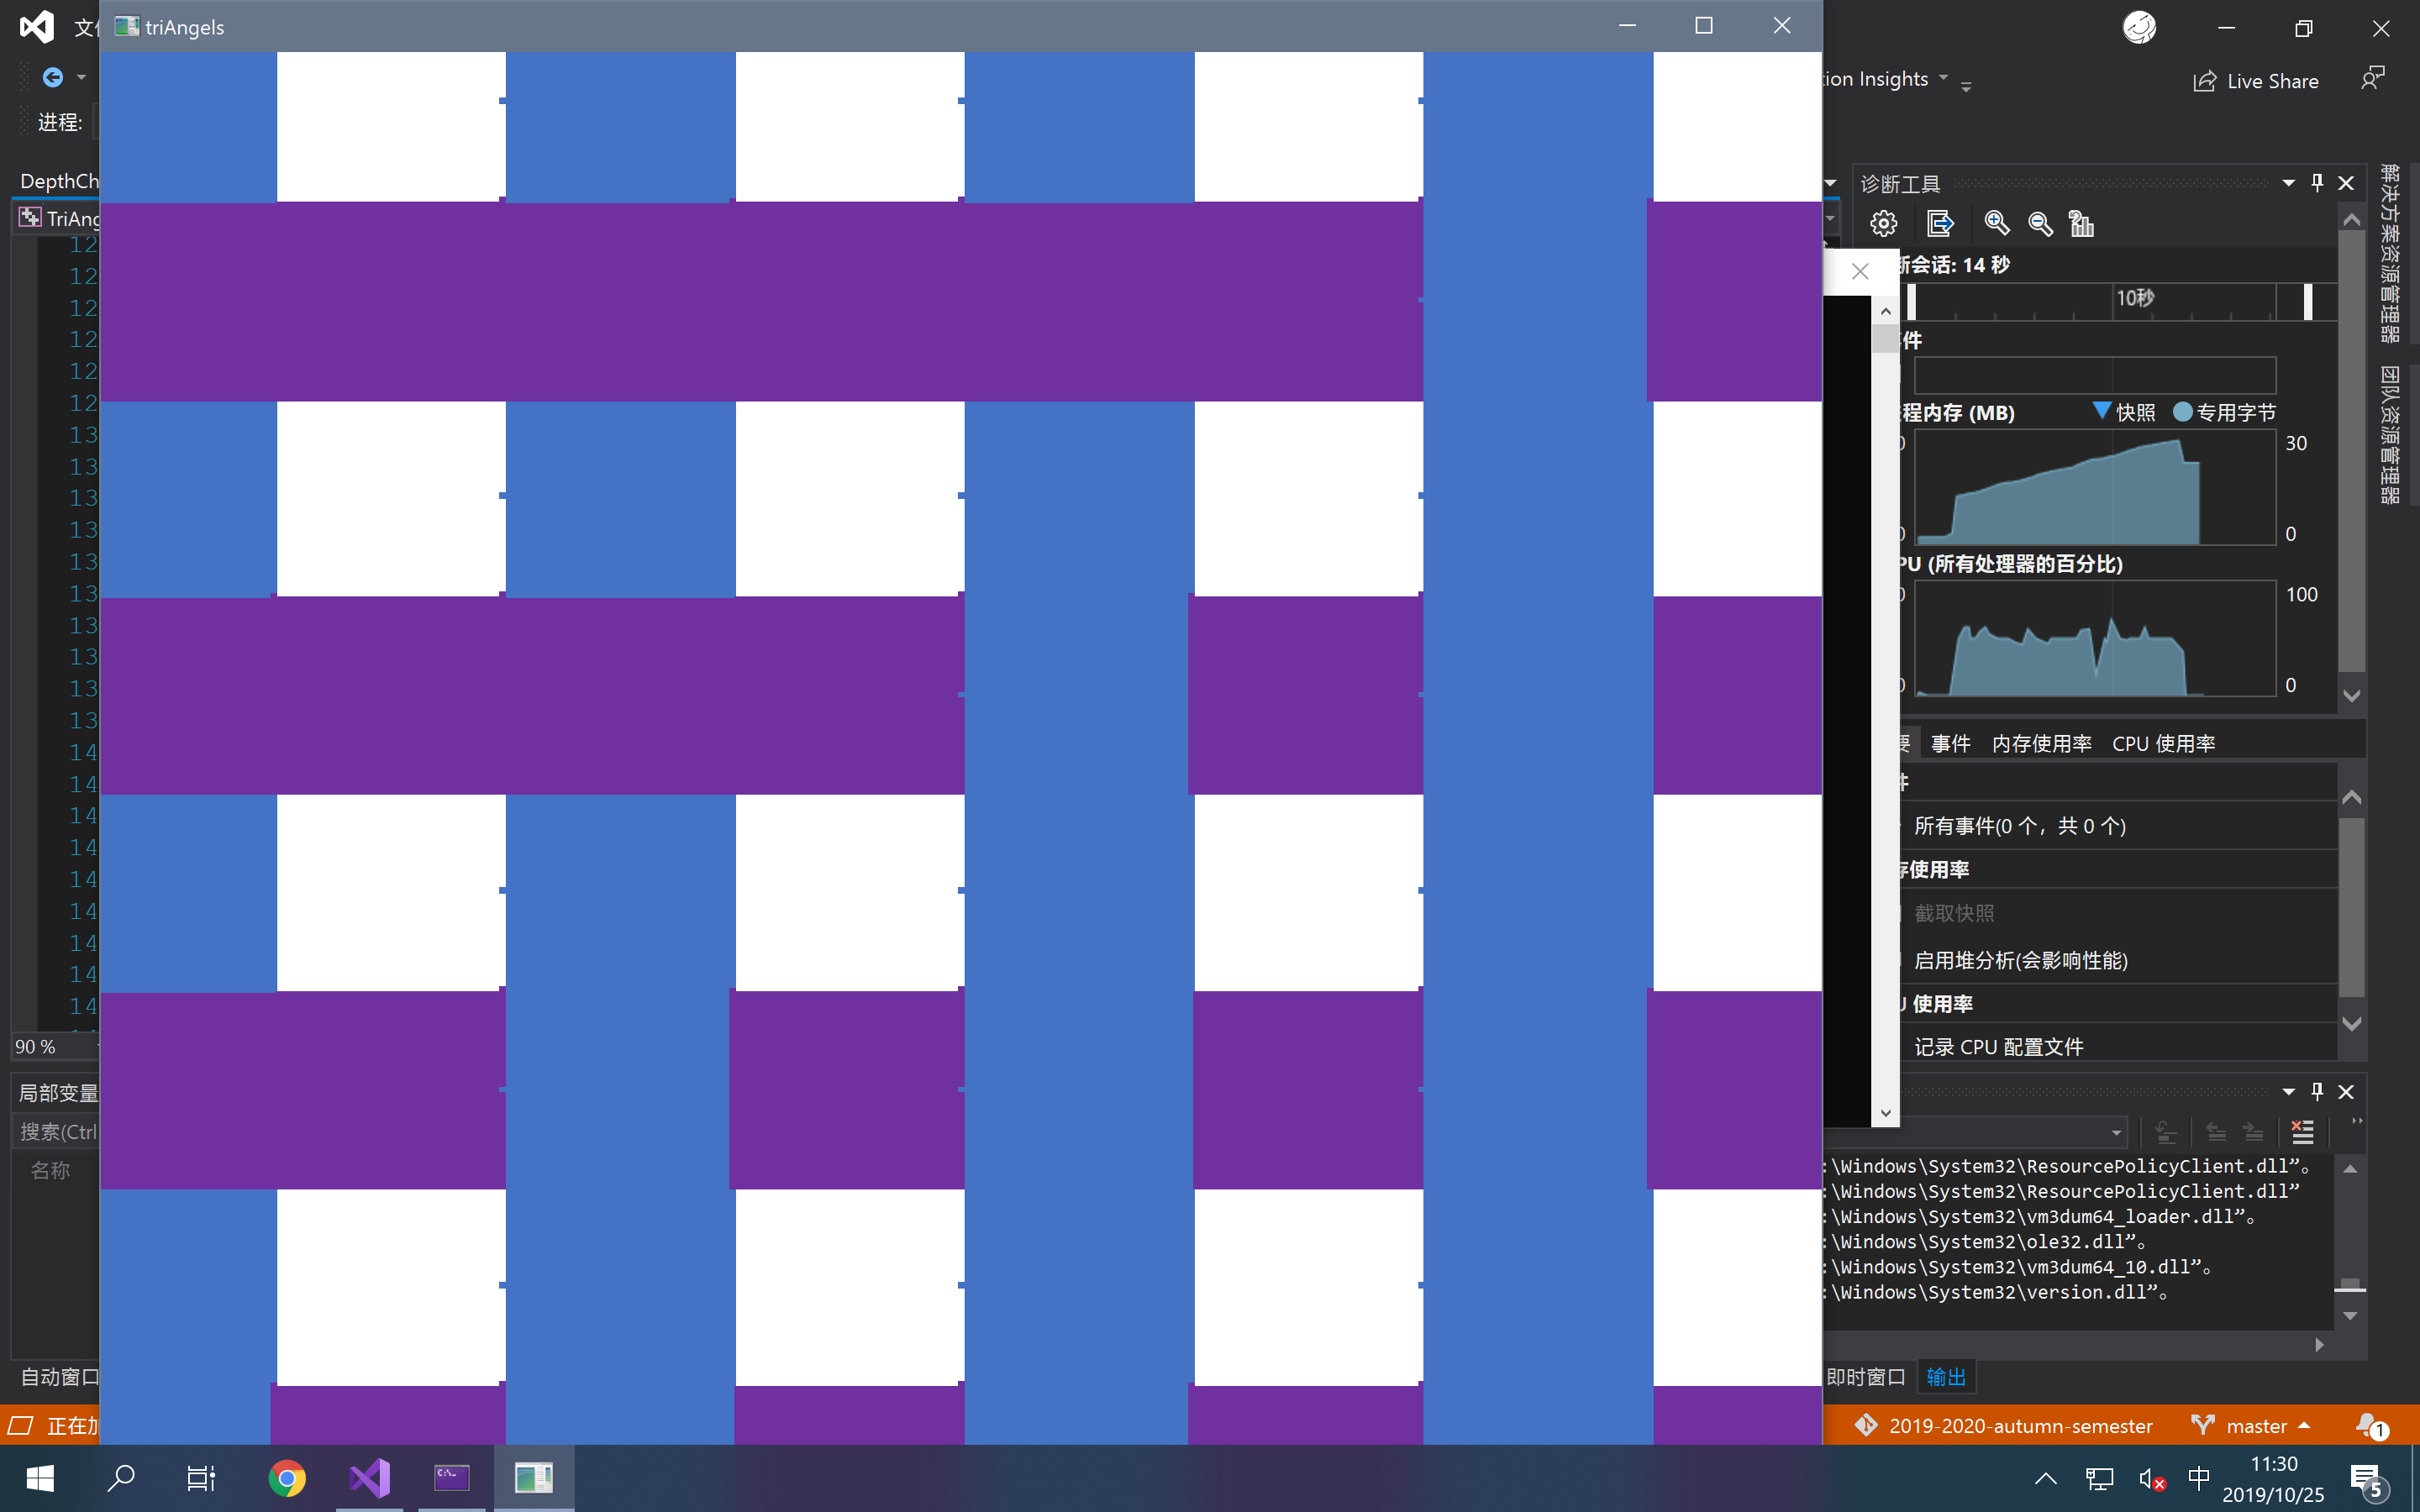
\includegraphics{/Users/yue/Documents/GitHub/2019-2020-autumn-semester/SE-344/submissions/ass2/screenshots/img.006.png}
\caption{}
\end{figure}

\begin{quote}
矩形编织效果,使用自定义的扫描线算法
\end{quote}

\begin{quote}
⚠️
注意:由于需要绘制的三角形较多,使用自定义扫描线方法渲染较慢,开启优化后在测试机器上大约需要
5 至 10 秒完成渲染。请耐心等待。
\end{quote}

\hypertarget{header-n179}{%
\subsubsection{笔记整理}\label{header-n179}}

\hypertarget{header-n180}{%
\paragraph{Sep 26}\label{header-n180}}

\begin{Shaded}
\begin{Highlighting}[]
\FunctionTok{## SE-344::CG2019}

\FunctionTok{### Review of Assignment #1}

\FunctionTok{### CG 发展 + 应用}

\FunctionTok{#### 發展}

\NormalTok{1946, ENIAC, 其创始人做了个梦…当时的 ENIAC 吃的是打孔纸带(输出也是),完全没有图形输出。}

\NormalTok{1950, MIT, Whirl Wind I 实现了第一台带显示器的计算机。用的是类似示波器的 CRT,只能显示非常简单的图形。}

\NormalTok{1958, Calcomp, 滚筒绘图仪。}

\NormalTok{1958, GerBer, 平板式绘图仪。}

\NormalTok{1960s, MIT, Lincoln Lab, 可交互的 CRT 显示器}

\NormalTok{>}\DataTypeTok{ 插一句:此时电视技术已经非常成熟了,因此也影响了计算机图形的发展历程。迄今为止,计算机图形技术都采用基于光栅的图形显示。}

\NormalTok{1980s, 出现了使用光栅图形显示器的 PC & Graphics Workstation。}

\NormalTok{>}\DataTypeTok{ 请注意:计算机图形所采用的 RGB 色域事实上并不能很好地表示出真实世界中的所有颜色。这个色域是比较窄的。图形工作站意在支持更多色彩的表示方式,实现真正的颜色「WYSIWYG」。}

\FunctionTok{#### 應用}

\NormalTok{* }\StringTok{Films,辅助影视后期制作。}
\StringTok{* Games,对于实时性的要求特别高。}
\StringTok{* Medical Imaging,医学图像学。}

\FunctionTok{### Graphics 的存储 + 表示 + 显示}

\NormalTok{表示和显示的区别:表示需要将所有的数据都表示出来,}
\NormalTok{然而显示的话仅仅显示那些必要的内容,很可能只有表示的数据(或者,实际的数据)的一部分。}

\NormalTok{例如:被空间遮挡的物体不会被显示;物体的一些信息:如法线等不会显示;}

\NormalTok{甚至,生成的图像也并非全部用于显示;一般会从生成的管线中进行剪裁(Clipping),这个图形显示的小窗口(Window)会因视点的位置(Viewpoint,视口)变换而变换。}

\NormalTok{>}\DataTypeTok{ 注意:此 Window 非彼 }\BaseNTok{`Windows`}\DataTypeTok{ 之 Window。}

\FunctionTok{#### 存儲}

\FunctionTok{#### 表示}

\NormalTok{图形是如何表示的?}

\NormalTok{这很难讲,主要是无法提出一个永远适用的标准来。}

\NormalTok{不同的应用场景总是会适用不同的表示方法。不同的物体也应该用不同的方式来表示。不能存在一个放四海准的统一标准。}

\NormalTok{在我们的 OpenGL 表示方法中,常用的表示方法是 顶点 三角形 上色。}

\NormalTok{三个顶点所构成的三角形都会被上成相同的颜色。在此基础上进行栅格化,确定到每个像素点应该取什么颜色。}

\FunctionTok{#### 顯示}

\NormalTok{在你知道了每个像素点的颜色之后,就可以交给 Graphics Card 来渲染了。}

\FunctionTok{### 图形处理管线}

\NormalTok{>}\DataTypeTok{ 也称渲染管线、渲染流水线, the rendering pipeline。}

\NormalTok{图形的显示本质上是以流水线来进行的。流水线的特点就是:其中一点的栓塞就会变成整体性能的瓶颈。因为其中每一级的产物都是下一级的必要输入。这样就会导致严重的卡顿和延迟。}

\NormalTok{管线里面有啥呢?}

\NormalTok{Geometry Pipeline ==光=栅=化=> Imaging Pipeline}

\FunctionTok{#### Geometry Pipeline}

\NormalTok{也叫做几何管线、3D 管线。这一段处理的都是 3D 空间内的顶点、边、光影、运动等等东西都是在此段进行考虑的。这一段还没有进行栅格化,操作的量都是矢量、几何量。}

\NormalTok{* }\StringTok{时间:动画与交互}
\StringTok{* 形状:建模}
\StringTok{* 着色:反射与光照}
\StringTok{* 视图:变换与剪裁}
\StringTok{* 消隐:隐藏线/隐藏面的消除}

\NormalTok{这些东西都是 G.P. 需要考虑的事情。}

\FunctionTok{#### 光栅化}

\NormalTok{光栅化就是 G.P => I.P. 的过程。这个过程是必然会导致大量信息丢失的。但是为了显示,不得不采用这种光栅化的操作。为了尽量减少损失,这里有非常大量的算法和操作,就是为了保留「真实感」。}

\NormalTok{>}\DataTypeTok{ 举例:一个几何管线里的球,如果你不加算法地渲染成二维,那肯定渲染成一个纯色的圆。}

\FunctionTok{#### Imaging Pipeline}

\NormalTok{此段已经把 Geometry pipeline 里面的几何数学量都采样、投影到 2D 平面,得到了一组像素化的 Pixels。}

\NormalTok{此时所有的光影、集合、3D 信息全部都丢失了。你得到的仅仅是一些平面像素颜色点。只能操作那些像素点了。}

\NormalTok{>}\DataTypeTok{ 为了尽量保留真实感,在 Imaging Pipeline 里面需要做的事情有:}

\NormalTok{* }\StringTok{光栅化、采样}
\StringTok{* 纹理映射}
\StringTok{* 图像合成}
\StringTok{* 光强、色彩量化}
\StringTok{* 帧缓存、显示}

\NormalTok{>}\DataTypeTok{ Question: 管线优化:能在哪里进行优化?如何找到哪里是瓶颈?如何优化?}

\FunctionTok{### 表示方法}

\FunctionTok{#### 线框模型}

\NormalTok{这个只能用来快速看一看,所有的面都不渲染,只渲染线条。问题就是会出现二义性,部分线条之间无法分析出来深度关系。}

\FunctionTok{#### 面模型}

\NormalTok{只渲染面,而被面遮挡的「内部」皆不渲染。}

\FunctionTok{#### 体表模型}

\NormalTok{用非常简单的几何体来代替我们的几何体,如四面体、六面体、球等等。}

\FunctionTok{#### 固定明暗}

\NormalTok{在上面这一步之后,已经有了一个非常粗略的视图。}

\NormalTok{所谓固定明暗,并非是「没有光源」。否则你渲染出来的就是一张黑帧。}

\NormalTok{而我们这一步里面要用到的是一种「不真实」的光;这种光让任何一点光强相同,且反射方式均为漫反射。}

\NormalTok{>}\DataTypeTok{ 同样亮度的漫反射啊,让人看起来真实感非常弱。}

\FunctionTok{#### Phong 光照模型}

\NormalTok{这一步比起上一步就是需要加入真实光照并加入渲染。}

\NormalTok{* }\StringTok{添加高光}

\NormalTok{在此之后物体会显得非常光滑,非常不真实(真实世界里没有这种油油亮亮的东西)}

\NormalTok{* }\StringTok{添加镜面反射}

\NormalTok{事实上反射并不好操作。实际有两种方法:}

\NormalTok{1. }\StringTok{用光线跟踪,遇到光反射的时候就反向追踪,找出光线的发射者,并计算反射的光强。这种算法计算量很大,而且在追踪距离较短时效果不好,容易出戏。}
\StringTok{2. 用帧缓存中上一帧渲染出来的结果拿出来,略加处理之后当纹理贴到镜子上(咳咳咳)}
\StringTok{3. A.O. 游戏里面特别常用的一种方法。}

\NormalTok{>}\DataTypeTok{ Question: 是啥?去查!}

\NormalTok{* }\StringTok{贴图}

\NormalTok{有些物体有特定的贴图,进行像素级别的计算。}

\NormalTok{* }\StringTok{凹凸映射}

\NormalTok{用纹理直接实现非常细小的凹凸变换,而不需要使用几何建模(细小的凹凸不平非常吃计算量的)。}
\NormalTok{而如果使用纹理来代替,可以用较小的代价实现几乎类似的效果。}
\end{Highlighting}
\end{Shaded}

\hypertarget{header-n182}{%
\paragraph{Oct 10}\label{header-n182}}

\begin{Shaded}
\begin{Highlighting}[]
\FunctionTok{## SE-344::Computer Graphics}

\NormalTok{不论你要 Build 出如何真实、如何帅气、如何有意思的图形,}

\NormalTok{最终你还是要把它给 Render, Flatten 成一个个无趣的像素点的。}

\NormalTok{这个过程就叫做「光栅化技术」。}

\NormalTok{---}

\FunctionTok{### 光栅化技術}

\NormalTok{光栅化之前所有的操作還可以包含 Vertex(頂點)、拓撲關係等等幾何信息;}

\NormalTok{但光栅化操作會把這些全部拍平;}

\NormalTok{光栅化之後的所有操作都只能基於 Pixels(像素點)了。}

\FunctionTok{#### 基本圖元繪製算法}

\NormalTok{我們要瞭解的僅僅就是基礎的算法原理而已。因為目前所有的基礎庫都很好地替我們提供了優秀的實現,我們不必要自己實現這些算法。}

\NormalTok{(雖然在下次作業裡,我們還是會需要做它一次。)}

\FunctionTok{#### 圖形的表示}

\NormalTok{* }\StringTok{WireFrame,線框模型}

\NormalTok{僅僅採用頂點和鄰邊來表示模型。}

\NormalTok{如果只有三維的線框模型的話,這種表示是存在二義性的。由於不存在遮擋關係,沒辦法唯一地表現出空間的。}

\NormalTok{只是快速表示一下空間而已。}

\NormalTok{* }\StringTok{Surface,表面模型}

\NormalTok{這種表示方法相較於 WireFrame,是由很多個 Surface(面片)搭建成的。由於面片之間存在遮擋關係,因此就表示精確度而言高於 WireFrame 模型。}

\NormalTok{但他沒有說明這圖形是由表面的哪一邊組成的。}

\NormalTok{* }\StringTok{Solid,實體模型}

\NormalTok{這種模型表示方法是可以定義形體處於表面的哪一側的。}

\NormalTok{還有很多種圖形的表示方法:}

\NormalTok{* }\StringTok{表面多邊形法(B-rep)}
\StringTok{* 解析法、微分法}
\StringTok{* 掃描表示法}
\StringTok{* 四叉樹、八叉樹表示法}
\StringTok{* 分形幾何法}
\StringTok{* 粒子系統(Particle System)}

\FunctionTok{#### 圖形的顯示}

\NormalTok{顯示跟表示是不一樣的。}

\NormalTok{顯示文件僅僅是整個圖形表示的一部分。}

\NormalTok{---}


\NormalTok{取景窗口也决定了显示的内容。这个取景窗口的决定叫做 Clipping。}

\NormalTok{* }\StringTok{每一个可以独立显示的点叫做像素点「Pixel Points」。}
\StringTok{* 一行像素构成一条光栅(Raster),也叫做扫描线(Scanline)。}

\NormalTok{确定屏幕上像素点的集合和颜色,叫做光栅化(Rasterization),也叫做扫描线算法(Scanline Algorithms)。}


\NormalTok{多年以前的 CRT 显示器需要扫描显示。因此它就有两种不同的扫描方法:}

\NormalTok{* }\StringTok{奇数场优先;}

\NormalTok{奇数场优先就是优先画出奇数场的扫描线,然后回扫;(回到第一个地方)而偶数场的扫描线就先暂且留在上一帧的位置。}

\NormalTok{* }\StringTok{偶数场优先;}

\NormalTok{和奇数场优先相反。}

\NormalTok{* }\StringTok{逐行显示}

\NormalTok{不区分上下/奇偶场。}

\FunctionTok{#### 帧缓冲存储器}

\NormalTok{存储器中包含了每个像素的信息。}

\NormalTok{拿出对应像素点的信息,放到对应的寄存器(Register)之中,然后送给显示控制器来干活;最终显示出来。}

\NormalTok{彩色的呢复杂一点。}

\NormalTok{有三个独立的显示控制器(R/G/B)共同显示彩色。}

\NormalTok{因此就需要三重显示控制器。}

\NormalTok{>}\DataTypeTok{ P.S. 部分的显示系统还包括了 Alpha 通道(也就是不透明度的控制)。但是并不存在一种「Alpha 显示控制器」。在此之前他就已经被平摊到 R/G/B 通道上了。}

\FunctionTok{### OpenGL 的基本图元绘制}

\FunctionTok{#### 定义顶点}

\NormalTok{顶点是一切东西的开始和基础。}

\NormalTok{由它才产生出了点、线、多边形,等等。}

\FunctionTok{##### `glVertex*`}

\NormalTok{>}\DataTypeTok{ }\BaseNTok{`*`}\DataTypeTok{ 代表这个函数有后缀。合理的后缀形似:}

\NormalTok{* }\StringTok{glVertex2i}

\NormalTok{2 代表这个顶点在二维空间之中。}

\NormalTok{i 代表这个点的坐标值为整数。}

\NormalTok{s 代表这个点的坐标值为段整数。}

\NormalTok{* }\StringTok{glVertex3f}

\NormalTok{3 代表这个顶点在三维空间之中。}

\NormalTok{f 代表这个点的坐标值为单精度浮点数。}

\NormalTok{d 代表这个点的坐标值为双精度浮点数。}

\NormalTok{以此类推。}

\BaseNTok{```c++}
\BaseNTok{glBegin(GL_POINTS);}

\BaseNTok{...}

\BaseNTok{glEnd();}
\BaseNTok{```}

\BaseNTok{`glBegin`}\NormalTok{ 和 }\BaseNTok{`glEnd`}\NormalTok{ 之间的部分就是我们定义的顶点们。}

\NormalTok{glBegin 中有一些参数,决定了怎么处理 glBegin 和 glEnd 之间定义的图元。}

\NormalTok{参数去看 PPT。这里记不下来。}

\FunctionTok{#### Example}

\BaseNTok{```c++}
\BaseNTok{glClear(GL_COLOR_BUFFER_BIT);}

\BaseNTok{glColor3f(0.2, 0.7, 0.7);}

\BaseNTok{glPointSize(5.0);}

\BaseNTok{glBegin(GL_POINTS);}

\BaseNTok{glVertex2f(0.0, 2.0);}

\BaseNTok{...}

\BaseNTok{glEnd();}

\BaseNTok{glFlush();}

\BaseNTok{```}

\NormalTok{P.S. 可以在 }\BaseNTok{`glBegin()`}\NormalTok{ 和 }\BaseNTok{`glEnd()`}\NormalTok{ 之间通过 }\BaseNTok{`glColor3f`}\NormalTok{ 来修改顶点的颜色。}

\NormalTok{不同的顶点颜色组装在一起会产生渐变颜色效果。这是双线性插值的结果。以后会讲到。}

\FunctionTok{### 基本图元光栅化算法}

\NormalTok{最基本的事情。我们都很关心。}

\FunctionTok{#### 啥是基本图元啊?}

\NormalTok{Primitive Symbols。什么算基本?}

\NormalTok{点、线、圆、一般函数曲线、字符。}

\FunctionTok{#### 光栅化/扫描线算法}

\NormalTok{把原来的一个美好的几何图形给拍扁成一堆像素点。}

\NormalTok{这个过程就是光栅化/扫描线算法。}

\FunctionTok{#### Fragment:片元}

\NormalTok{光栅化完成之后,原来那个图元对应的像素点集合就叫片元区域。}

\FunctionTok{#### 光栅化}

\FunctionTok{##### 点的光栅化}

\NormalTok{P(x0, y0) 怎么变呢?}

\NormalTok{>}\DataTypeTok{ 法一:直接取整数部分。}

\NormalTok{>}\DataTypeTok{ 法二:四舍五入。}

\NormalTok{这两者区别不太大,但是总的来说四舍五入的像素点偏移会更少。}

\NormalTok{如果说直接取整数部分,有可能会产生整体像左下角(0, 0 位置)的偏移。}

\NormalTok{但总归,点的光栅化都是容易的。}

\FunctionTok{##### 直线的光栅化}

\NormalTok{在数学中,直线的斜截式方程为 $y = k x + b$。}

\NormalTok{但事实上计算机不会处理无限长的直线。它只会处理有限的线段。}

\NormalTok{因此我们一般会提供起点和终点 P1(x1, y1) - P2(x2, y2)。只画这两点构成的线段。}

\NormalTok{平凡的四种线段:$y = k$,$x = k$,$x = y$,$x = -y$。这个光栅化过于简单,不多谈。}

\NormalTok{我们可以直接把它简化为点的光栅化问题。把这个线段给切分成一些点的集合(按照一定的切分粒度),然后对每一个点进行光栅化。}

\NormalTok{在斜率 k 绝对值小于 1 的时候就用变化的 x 来求 y。}

\NormalTok{在 k 绝对值大于 1 的时候就用变化的 y 来求 x。}

\NormalTok{但这个算法非常之慢。正常人类不会用的。}

\FunctionTok{##### 直线的光栅化(人类的方法)}

\NormalTok{DDA 算法:Digital Difference Algorithm。}

\NormalTok{这是一个增量计算法;也就是每一步计算都跟上一步的计算结果有关系。}

\NormalTok{我们知道起点和终点;先把起点给光栅化掉再说。}

\NormalTok{然后我们就有了另一个参量:当前绘制的点。}

\NormalTok{我们判断这个当前点是偏向了 y 轴(向上偏了)还是偏向了 x 轴(向下偏了)。}

\NormalTok{如果斜率偏小,那下一步就往右走;如果斜率偏大,那下一步就往上走。}

\NormalTok{如果不偏不倚;刚好一样,那就往右上方走。}

\NormalTok{这么办可以保证比较高的效率,同时 trivial 的四种情况也可以直接处理掉。}

\NormalTok{当然这种方法就仅仅适用于直线而已。其他的曲线是不可以用的。}

\NormalTok{附注:一般来说结尾点我们是不画的。因为经常会画连续的方法;}

\FunctionTok{##### 直线的光栅化(Bresenham 算法)}

\NormalTok{这个方法太快啦!所以它也被叫做「快速增量算法」。}

\NormalTok{基本思想是根据一个决策项 p 的正负,来选择像素点的位置。}

\NormalTok{本质上,需要在 x 方向上移动 A 格,同时在 y 方向上移动 B 格。}

\NormalTok{那么我们只需要决定在什么时候往右走,在什么时候往上走,就好了。}

\NormalTok{不需要进行那么多次的除法运算(说的就是 DDA),}

\NormalTok{思路是绝对的简单:我可以选择的像素点位置谁离真实值比较近,我就选谁走。}

\NormalTok{本算法所需要进行的计算仅仅包括「×2」和「-」。对应到位运算就是仅仅包括左移一位和减法器。}

\NormalTok{比起那些动不动要乘要除的浪费 CPU Cycle 的那些算法,这个算法简直太快了!}

\FunctionTok{##### 圆的光栅化}

\NormalTok{圆有二次多项式表示。}

\NormalTok{圆也有极坐标表示。}

\NormalTok{圆也有 Brosenham 栅格化算法。}

\NormalTok{看书 P110.}
\end{Highlighting}
\end{Shaded}

\hypertarget{header-n184}{%
\paragraph{Oct 17}\label{header-n184}}

\begin{Shaded}
\begin{Highlighting}[]
\FunctionTok{## SE-344::CG}

\NormalTok{终极目标:得到一帧可显示的图像。其中最重要的一个步骤就是光栅化了。}

\NormalTok{每一个像素格的颜色都放在一个叫做「帧缓冲存储器」的东西里。}

\NormalTok{OpenGL 里如何定义那些点及其他基本图元,我们也已经了解到了。}

\NormalTok{关于点和线这种图元的光栅化所用到的各种算法,我们上节课也讲了。}

\NormalTok{光栅化完了之后,得到的像素点集合就改名叫 Fragments(片元)了。}

\FunctionTok{### 多边形的光栅化}

\NormalTok{多边形其实也是 Primitive 的一种的。但是他的光栅化比起点跟线来说,相对更难一些。}

\FunctionTok{#### **最**低效法}

\NormalTok{逐个检查像素是否在多边形内。丢人!谁会用这种方法}

\FunctionTok{#### 空间连贯性利用法}

\NormalTok{相邻像素几乎都具有相同的填充状态,只需要在边缘位置进行特别检查和处理。}

\NormalTok{#####基本步骤}

\NormalTok{* }\StringTok{求扫描线与多边形边缘的交点}
\StringTok{* 对交点排序,分块}
\StringTok{* 确定每一块 Span 的填充状态}
\StringTok{* 处理特别状态:扫描线掠过顶点时怎么处理}

\FunctionTok{##### 特别说明}

\NormalTok{为了解决「填充扩大」问题,采用「右上闭左下开」原则,确保多边形绘制结果不扩大。}

\FunctionTok{#### 奇偶扫描转换算法}

\NormalTok{由上面的空间连贯性扫描线大法衍生而来。每根扫描线存有一个 Bit 标识位,在进入/离开多边形边缘时切换奇偶标识位,并以此标识位决定要不要画像素。}

\NormalTok{这种算法利用了水平方向的连续性,但却没有用好竖直方向的大体相似性,所以效率有点感人。}

\FunctionTok{#### 有序边表多边形扫描转换算法}

\NormalTok{这种方法的思路是首先计算出所有的端点及其与扫描线的交点,然后两两取出成对的点构成线段并光栅化。最后得到结果。}

\FunctionTok{#### 采用活化边表的有序边算法}

\NormalTok{活化边表:不仅仅采用从上到下的扫描顺序,而是根据当前扫描线的位置动态改变边表的内容及顺序,某些根本碰不到扫描线的边就直接从活化边表中剔除,这样可以减少比较次数,提升一定的效率。}

\FunctionTok{#### 边填充算法}

\NormalTok{每一条跟多边形相交的扫描线,将其交点取为 $(x1, y1)$,把每一条边靠近图形内侧的像素点都填上,最后取交集得到结果。}

\NormalTok{这个效率是真的很低(×)}

\FunctionTok{#### 栅栏填充算法}

\NormalTok{所谓 Fence 填充,就是提供一个人为限定的边界,减少那些「不可能」的像素点被 Call 的次数,大大减少了像素点访问次数。稍微提高了点效率。}

\NormalTok{但还是差(×)}

\FunctionTok{#### 边标识算法}

\NormalTok{终于有一种适合硬件实现的、好使的算法了(}

\NormalTok{沿着多边形勾画轮廓线,建立各区段的像素的时候,同时把它们之间的像素也都填上。}

\NormalTok{这种算法每个像素点访问至多一次。很高效。}

\FunctionTok{#### 种子填充算法}

\NormalTok{首先指定一个已知在多边形内部的像素点,然后四处找邻居扩散;遇到了边界像素,就撞墙碰壁停止;}

\FunctionTok{##### 4 连通法}

\NormalTok{只有上下左右的作为邻居。}

\FunctionTok{##### 8 连通法}

\NormalTok{除了上下左右,右上右下左上左下也可以当作邻居。}

\NormalTok{通过这种方法,扩散开来填充整个多边形。}

\NormalTok{一般这种算法用个 Stack 就好了。用递归太浪费,算了。(本质上也是用一个 Callee Stack...)}

\FunctionTok{#### 扫描线种子填充算法}

\NormalTok{不采用唯一一个像素点来开始种子填充,而是使用一根扫描线找出内部像素全部扔入栈,然后向两边扩展开。}

\FunctionTok{#### 泛滥填充算法}

\NormalTok{(???)这是啥}

\NormalTok{没有特定边界,把图像中所有满足一定颜色范围的像素点都修改为同一颜色,而不考虑其空间分布。}

\FunctionTok{#### 渐变填充算法}

\NormalTok{(???)好像跑偏了}

\NormalTok{先确定好他是否是存在于多边形内部的点。然后给定边缘点的颜色,内部其他点的颜色都采用双线性插值确定。}

\NormalTok{以 $(C1, C2, C3)$ 为例,三个点确定的一个三角形,给这三个点指定三种不同的颜色。}

\NormalTok{那么对于三角形内部任意一点 $P(x, y)$ 而言,计算出他与三角形的两个交点 $P1(x1, y)$ 和 $P2(x2, y)$。在这条扫描线上,我们认定颜色值就是线性变化的。所以我们只要知道 P1 跟 P2 的颜色值,就可以直接拿到结果了。}

\NormalTok{那么 P1 跟 P2 的颜色值怎么确定呢?因为 P1 跟 P2 都在直线边界上,所以我们只需要把它的 x 或 y 坐标拿出来同这条边两边的两个端点拿来做插值就可以了!}

\NormalTok{很简单的一种算法。}

\NormalTok{>}\DataTypeTok{ Première}

\FunctionTok{### OpenGL 多边形填充}

\FunctionTok{#### 顶点数据的维护}

\NormalTok{#####立即模式}

\NormalTok{~~猴急模式~~}

\NormalTok{现在几乎没什么人用这种方法了。每创建一个顶点就把它立即发给显卡画。效率是比较低的。}

\NormalTok{#####VBO/VAO}

\NormalTok{VBO 是 Vertex Buffer Object 的简称。显卡内的一个内存缓冲区,可以保存顶点、颜色、法线、纹理等等信息。这些信息都还是光栅化之前的图形数据。}

\NormalTok{VAO 是 Vertex Array Object 的简称。一个 VAO 包含一个或多个 VBO。VAO 会在显存之中线性存储几个对象信息,而不是直接每次都把每一个对象数据发给显卡。这就是 Non-Instant 非立即模式下的工作方法。}

\FunctionTok{#### 指定颜色及其填充方式}

\NormalTok{使用 }\BaseNTok{`glColor*\{*\}()`}\NormalTok{ 来指定每个顶点的颜色。}

\NormalTok{使用 }\BaseNTok{`glShadeModel(GLenum mode)`}\NormalTok{ 来确定颜色的填充方法。}

\BaseNTok{`GL_SMOOTH`}\NormalTok{:缺省值。使用双线性插值来确定颜色。}

\BaseNTok{`GL_FLAT`}\NormalTok{:采用离该点最近的顶点的颜色作为该点的颜色。}

\FunctionTok{#### 指定多边形绘制方式}

\NormalTok{使用 }\BaseNTok{`glPolygonMode(GLenum face, GLenum mode)`}\NormalTok{ 来确定多边形的绘制方式。}

\NormalTok{Face 的取值范围:}

\BaseNTok{`GL_FRONT`}\NormalTok{、}\BaseNTok{`GL_BACK`}\NormalTok{、}\BaseNTok{`GL_FRONT_AND_BACK`}\NormalTok{,确定对于一个多边形来说是绘制它的正面、背面还是两面都绘制。}

\NormalTok{Mode 的取值范围:}

\BaseNTok{`GL_POINT`}\NormalTok{ 点填充,只画你说的那几个点}

\BaseNTok{`GL_LINE`}\NormalTok{ 帮你把边给连上}

\BaseNTok{`GL_FILL`}\NormalTok{ 缺省值,帮你填充上多边形。}

\FunctionTok{#### 指定多边形的正反面}

\BaseNTok{`glFrontFace(GL_CCW / GL_CW)`}\NormalTok{ 函数可以做到制定多边形的正面反面。}

\NormalTok{缺省情况下以右手系作为世界坐标系,逆时针成的面作为正面。}

\NormalTok{总归记住:面和边都是有方向的。}

\FunctionTok{#### 指定图案填充多边形}

\BaseNTok{`glPolygonStipple(const GLubyte *mask)`}\NormalTok{ 可以用来图案填充多边形。 }

\FunctionTok{### 可见面判别算法}

\FunctionTok{#### 图形的二义性}

\NormalTok{在投影变换之后,3D 变 2D 之后,深度信息就丢失了,可能同一种投影会产生多种可能的原图形。}

\NormalTok{那么为了正确地绘制出无二义性的图形,深度信息必不可少。}

\NormalTok{复杂的情况下,一个图形本身的面、不同的物体之间都会产生遮挡。正确渲染这些面就必须要有深度信息加持。}

\FunctionTok{#### 判定法}

\FunctionTok{##### 画家算法(Naïve 算法)}

\NormalTok{类似于油画的作画过程;首先把屏幕设定为背景色。然后按照各个面按照视觉距离排序;于是先绘制远景、再画中景;最后画近景。类似于油画颜料的可覆盖性。}

\NormalTok{问题:一个像素需要被画很多次,效率很低。况且可能有些面可能会倾斜,可能会相交。并不能很好地进行排序。}

\FunctionTok{##### 后向面}

\NormalTok{或称背向面。指当前视点对应的观察方向所看不到的那些面。}

\FunctionTok{##### 后向面判别算法}

\NormalTok{设当前观察方向为 $V$,同一个坐标系下,多边形面的法矢为 $N(xn, yn, zn)$。将他们做点乘,在 $V·N>0$ 时,认定他为后向面,隐藏它并不做显示。}

\FunctionTok{##### 深度缓冲器算法}

\NormalTok{或称作 Depth Buffer Method, Z-Buffer Method.}

\NormalTok{典型的像空间算法。}

\NormalTok{对场景中每个物体的每个表面进行处理,对比出深度最大的表面进行显示。}

\NormalTok{######初始化}

\NormalTok{$depth(x, y) = 0$。$refresh(x, y) = I(backend)$。}

\FunctionTok{###### 比较}

\NormalTok{存储比较每个多边形上各点的深度值,并进行可见性判断}

\FunctionTok{###### 计算}

\NormalTok{计算各个点 $(x, y)$ 处的深度值 $z$;}

\FunctionTok{###### 结果}

\NormalTok{若 $z > depth(x, y)$,则有}

\NormalTok{$$depth(x, y) = z; refresh(x, y) = I(surf)(x, y)$$}

\FunctionTok{##### A 缓冲器算法}

\NormalTok{上面的 DBM 法只能找到一个可见面,也就是说只能处理非透明的表面。没办法处理混合光强值。}

\NormalTok{对深度缓冲器算法进行了一点扩充:每一个位置都对应着一个 Surface Linked List。链表里就有了当前 Surface 之后的面的信息了。有了这些信息,我们就可以处理光强混合、半透明表面之类的操作了。}

\FunctionTok{##### 扫描线算法}

\NormalTok{可以处理表面相交的情况了!}

\FunctionTok{##### 光线投影算法}

\FunctionTok{### 反走样技术}

\NormalTok{Anti-Aliasing Technique}

\NormalTok{CG 总是会走样的。但我们能不能稍微挽救一下?}

\FunctionTok{#### 采样}

\NormalTok{>}\DataTypeTok{ Sampling}

\NormalTok{走样源自于采样。}

\NormalTok{采样就是把连续数据转变为离散信息的过程。这就是数据丢失的过程啊。}

\NormalTok{>}\DataTypeTok{ 走样 *zǒuyàng* **动**}
\DataTypeTok{>}
\DataTypeTok{> 失去了原来的样子。}
\DataTypeTok{>}
\DataTypeTok{> *这双鞋没穿几天就走样了 | 贯彻会议精神不走样。*}

\NormalTok{采样过程中会失真。失真过于明显,产生走样。}

\FunctionTok{#### Nyquist 采样定理}

\NormalTok{要想从采样信息中重建原始信号,则采样频率必须大于等于原始信号最大频率的两倍。}

\FunctionTok{#### 反走样技术}

\NormalTok{用于减少或消除走样效果的技术。也称为抗锯齿算法。也称为 Anti-Aliasing 算法。也称为 AA。}

\FunctionTok{#### 图形反走样}

\FunctionTok{##### 基础思路}

\NormalTok{把像素作为一个区域,按照区域进行采样。}

\NormalTok{按照我们栅格化图形的过程中,有的格子是部分落在原图形中的。我们按照占有的比率对其进行灰度级别上色,可以改善人眼的视觉体验。}

\FunctionTok{##### 操作}

\NormalTok{给定一个最大亮度值,代表完全被覆盖的情况下所对应的颜色。}

\NormalTok{而那些被部分覆盖的像素点的亮度值设定为(覆盖百分比 × 最大亮度值)。}

\FunctionTok{##### 问题}

\NormalTok{* }\StringTok{无论像素距离图形有多远,相同的相交面积产生相同的亮度。也就是说离直线的距离这个因素并没有加权。因此还是有比较明显的锯齿效应。}
\StringTok{* 直线上的相邻像素点可能产生较大的灰度差。}

\FunctionTok{#### FSAA}

\NormalTok{全屏反走样技术,Full-Scene Anti-Aliasing。}

\NormalTok{主要针对 3D 场景的绘制。通过密集的采样和滤波来减少锯齿效应。}

\NormalTok{FSAA 在渲染一个实际区域的时候(如 1024 × 768)的时候,会事先计算出多倍大小的画面内容(如 4× 抗锯齿,会渲染出 2048 × 1536 的画面),通过密集的采样来进行全屏幕反走样操作。}

\FunctionTok{#### SS}

\NormalTok{Super Sampling,超级采样。}

\NormalTok{一个像素当作好几个像素来进行采样。那些「几个像素」就叫做「子像素」(Subpixels)。}

\NormalTok{渲染的时候场景放大渲染,但是以低分辨率进行显示。低分辨率下每一个像素都是多个像素加权平均的结果。}

\NormalTok{代价很高。真的很高。}

\FunctionTok{#### OGSS, RGSS, MSAA, Quincunx}

\NormalTok{SS 的几种实现。}

\NormalTok{OGSS:顺序栅格采样,按照 x、y 顺序进行采样。}

\NormalTok{RGSS:旋转栅格采样。}

\NormalTok{MSAA:多级采样技术,多边形内部无需超采样,因此 MSAA 只在边缘进行超采样,可以节约点时间。}

\NormalTok{Quincunx:五点梅花采样。每个点的颜色都跟自己周边的颜色有关,且分配有不同的权重。}
\end{Highlighting}
\end{Shaded}

\hypertarget{header-n186}{%
\subsubsection{问题提出与解决}\label{header-n186}}

\hypertarget{header-n187}{%
\paragraph{Q1:管线优化}\label{header-n187}}

在我们进行管线优化的过程中,如何找到哪里才是性能瓶颈(Bottleneck)?

\hypertarget{header-n189}{%
\paragraph{A1}\label{header-n189}}

由于 Pipeline 是一个有着严格先后顺序的流水线作业,因此其中任何一个环节的
throttle 都会导致整体的性能下降。

因此在我们进行优化的时候,可以依次从前到后对每一个环节的入时间和出时间进行计算,统计出其所占整体时间的比率,按照其满载比空载的时间比来确定哪一段占用了最长时间。

这样,针对耗时最长的片段进行优化就能取得较为显著的效果。

\hypertarget{header-n193}{%
\paragraph{Q2:AO}\label{header-n193}}

在游戏开发中常用的一种「A.O.」技术为何?

\hypertarget{header-n195}{%
\paragraph{A2}\label{header-n195}}

A.O.,全称为 Ambient Occlusion,即环境光遮罩。

为了在游戏开发中实现光找效果,我们有许多方法。其中主要的计算方法分为两种:直接光照与间接光照。

直接光照:仅仅考虑光线照在物体上然后直接反射到观察点的这部分光照信息。

间接光照:同时计算光线经过物体多次反射、折射、吸收之后的光线信息。

最优的解决方案当然是真实的进行全部计算;目前热门的「光线追踪」技术就是基于间接光照的思路来的。而在硬件没有提供支持的情况下,软件强行计算的效率是很低的。

因此 Unity
等游戏引擎提供了一个折中方案:依然还是按照直接光照的思路进行计算,而同时在每个取样点上计算它被其它几何体覆盖的程度,以此为根据调整其反射光线的强度,能够在一定程度上模拟出「亮度衰减」的效果。本质上也是一个在算力不充分的时期所进行的妥协。

\end{document}
